%%
%% This is file `sample-sigconf.tex',
%% generated with the docstrip utility.
%%
%% The original source files were:
%%
%% samples.dtx  (with options: `sigconf')
%% 
%% IMPORTANT NOTICE:
%% 
%% For the copyright see the source file.
%% 
%% Any modified versions of this file must be renamed
%% with new filenames distinct from sample-sigconf.tex.
%% 
%% For distribution of the original source see the terms
%% for copying and modification in the file samples.dtx.
%% 
%% This generated file may be distributed as long as the
%% original source files, as listed above, are part of the
%% same distribution. (The sources need not necessarily be
%% in the same archive or directory.)
%%
%% The first command in your LaTeX source must be the \documentclass command.
\documentclass[sigconf]{acmart}



%%
%% \BibTeX command to typeset BibTeX logo in the docs
\AtBeginDocument{%
  \providecommand\BibTeX{{%
    \normalfont B\kern-0.5em{\scshape i\kern-0.25em b}\kern-0.8em\TeX}}}




%% Rights management information.  This information is sent to you
%% when you complete the rights form.  These commands have SAMPLE
%% values in them; it is your responsibility as an author to replace
%% the commands and values with those provided to you when you
%% complete the rights form.
\setcopyright{acmcopyright}
\copyrightyear{2021}
\acmYear{2021}
\acmDOI{....}
%%\acmDOI{10.1145/1122445.1122456}

%% These commands are for a PROCEEDINGS abstract or paper.
\acmConference[Philadelphia '21]{Philadelphia '21: ACM Symposium on Parallelism in Algorithms and Architectures}{July 06--08, 2021}{Philadelphia (Online), USA}
\acmBooktitle{Philadelphia '21: ACM Symposium on Parallelism in Algorithms and Architectures,
  July 06--08, 2021, Philadelphia (Online), USA}
%%\acmPrice{15.00}
%%\acmISBN{978-1-4503-XXXX-X/18/06}
\acmPrice{0.00}
\acmISBN{XXXXX-XXXX-X/21/07}


%%
%% Submission ID.
%% Use this when submitting an article to a sponsored event. You'll
%% receive a unique submission ID from the organizers
%% of the event, and this ID should be used as the parameter to this command.
%%\acmSubmissionID{123-A56-BU3}

%%
%% The majority of ACM publications use numbered citations and
%% references.  The command \citestyle{authoryear} switches to the
%% "author year" style.
%%
%% If you are preparing content for an event
%% sponsored by ACM SIGGRAPH, you must use the "author year" style of
%% citations and references.
%% Uncommenting
%% the next command will enable that style.
%%\citestyle{acmauthoryear}

%%
%% end of the preamble, start of the body of the document source.

\usepackage[utf8]{inputenc}
%%%%\usepackage[cmex10,fleqn]{amsmath}
%%\usepackage{amsfonts}
%%\usepackage{amssymb}
\usepackage{amsmath}
\usepackage{amsfonts,amssymb,amsthm}
%%\usepackage{amsfonts,amssymb,amsthm}
\usepackage{graphicx}
\usepackage{color}
\usepackage{todonotes}
%%\usepackage{algorithm,algpseudocode}
\usepackage{algorithm}
\usepackage{algorithmic}
%%\usepackage{algcompatible}
\usepackage[position=below]{subfig}
\usepackage{xspace}
\usepackage{etoolbox}
\usepackage{xcolor}
\usepackage{multirow}
\usepackage{subfig}
\usepackage{balance}


%% uncomment the below line to remove all todos
\renewcommand{\todo}[2][1=]{}

\setlength{\tabcolsep}{2pt}

\definecolor{pdfurlcolor}{rgb}{0,0,0.6}
\definecolor{pdfcitecolor}{rgb}{0,0.6,0}
\definecolor{pdflinkcolor}{rgb}{0.6,0,0}

%%\usepackage[colorlinks=true,citecolor=pdfcitecolor,urlcolor=pdfurlcolor,linkcolor=pdflinkcolor,pdfborder={0 0 0}]{hyperref}
%%\usepackage[breaklinks]{hyperref}
%%\usepackage{subcaption}

\usepackage{tikz}
\usetikzlibrary{matrix, decorations, patterns, positioning, shapes, calc, intersections, arrows, fit}

\graphicspath{{./diagrams/}{./plots/}}

%%\theoremstyle{plain}
%%\newtheorem{lemma}{Lemma}
%%\newtheorem{theorem}{Theorem}
%%\newtheorem{proposition}{Proposition}
%%\newtheorem{corollary}{Corollary}
%%\newtheorem{definition}{Definition}



\newcommand{\tensor}[1]{{\cal\textbf{#1}\xspace}}
\newcommand{\ttrain}{{\it Tensor-Train}\xspace}

\newcommand{\hfirst}{{\it LSR}\xspace}
\newcommand{\hsecond}{{\it SLSB}\xspace}
\newcommand{\hthird}{{\it LSB}\xspace}
\newcommand{\otta}{{\it STTA}\xspace}

%%\setlength{\mathindent}{0pt}

%% Colors from https://latexcolor.com/
\definecolor{pastelviolet}{rgb}{0.8, 0.6, 0.79}
\definecolor{babyblueeyes}{rgb}{0.63, 0.79, 0.95}
\definecolor{pastelyellow}{rgb}{0.99, 0.99, 0.59}
\definecolor{pastelgreen}{rgb}{0.47, 0.87, 0.47}
\definecolor{pastelred}{rgb}{1.0, 0.41, 0.38}
\colorlet{patternblue}{blue!60}


\makeatletter
\DeclareRobustCommand*\cal{\@fontswitch\relax\mathcal}
\makeatother

\begin{document}

%%
%% The "title" command has an optional parameter,
%% allowing the author to define a "short title" to be used in page headers.
\title{Parallel Tensor Train through Hierarchical Decomposition}

%%
%% The "author" command and its associated commands are used to define
%% the authors and their affiliations.
%% Of note is the shared affiliation of the first two authors, and the
%% "authornote" and "authornotemark" commands
%% used to denote shared contribution to the research.
%%\author{Ben Trovato}
%%\authornote{Both authors contributed equally to this research.}
%%\email{trovato@corporation.com}
%%\orcid{1234-5678-9012}
%%\author{G.K.M. Tobin}
%%\authornotemark[1]
%%\email{webmaster@marysville-ohio.com}
%%\affiliation{%
%%  \institution{Institute for Clarity in Documentation}
%%  \streetaddress{P.O. Box 1212}
%%  \city{Dublin}
%%  \state{Ohio}
%%  \country{USA}
%%  \postcode{43017-6221}
%%}

%%\author{Laura Grigori}
%%\affiliation{%
%%  \institution{Alpines, Inria Paris\\
%%  	Sorbonne Université, Université de Paris\\
%%  	CNRS, Laboratoire Jacques-Louis Lions}
%%  \city{Paris}
%%  \country{France}}
%%\email{laura.grigori@inria.fr}
%%
%%\author{Suraj Kumar}
%%\affiliation{%
%%	\institution{Alpines, Inria Paris\\
%%		Sorbonne Université, Université de Paris\\
%%		CNRS, Laboratoire Jacques-Louis Lions}
%%	\city{Paris}
%%	\country{France}}
%%\email{suraj.kumar@inria.fr}

\author{Author1}
\affiliation{%
  \institution{ABC}
%%  \city{Paris}
  \country{XXXX}}
%%\email{laura.grigori@inria.fr}

\author{Author2}
\affiliation{%
	\institution{ABC}
	%%  \city{Paris}
	  \country{XXXX}}
	%%\email{laura.grigori@inria.fr}

%%
%% By default, the full list of authors will be used in the page
%% headers. Often, this list is too long, and will overlap
%% other information printed in the page headers. This command allows
%% the author to define a more concise list
%% of authors' names for this purpose.

\renewcommand{\shortauthors}{Author1 and Author2.}

%%
%% The abstract is a short summary of the work to be presented in the
%% article.
\begin{abstract}
We consider the problem of developing parallel decomposition and approximation 
algorithms for high dimensional tensors. We focus on a tensor representation 
named Tensor Train (TT). It stores a $d$-dimensional tensor in 
$\mathcal{O}(nr^2d)$, much less than the $\mathcal{O}(n^d)$ entries in the 
original tensor, where $r$ is usually a very small number and depends on the 
application. Sequential algorithms to compute TT decomposition and 
TT approximation of a tensor have been proposed in the literature. Here we 
propose a parallel algorithm to compute TT decomposition of a tensor. We prove 
that the ranks of TT-representation produced by our algorithm are 
bounded by the ranks of unfolding matrices of the tensor. Additionally, we 
propose a parallel algorithm to compute approximation of a tensor in 
TT-representation. Our algorithm relies on a hierarchical partitioning of the 
dimensions of the tensor in a balanced binary tree shape and transmission 
of leading singular values of associated unfolding matrix from the parent to 
its children. We consider several approaches on the basis of 
how leading singular 
values are transmitted in the tree. We present an in-depth experimental 
analysis of our approaches for different low rank tensors and also assess them 
for tensors 
obtained from quantum chemistry simulations. Our results show that the approach 
which transmits leading singular values to both of its children performs better 
in practice. Compression ratios and accuracies of the approximations obtained 
by our approaches are comparable with the sequential algorithm and, in some 
cases, even better than that. We also show that our algorithms transmit only $\mathcal{O}(\log^2 P\log d)$ number of messages along the critical path for a $d$-dimensional tensor on $P$ processors. The lower bound on the number of  messages for any algorithm which exchanges data on $P$ processors is $\Omega(\log P)$, and our algorithms achieve this bound, modulo polylog factor.
\end{abstract}

%%
%% The code below is generated by the tool at http://dl.acm.org/ccs.cfm.
%% Please copy and paste the code instead of the example below.
%%
%%\begin{CCSXML}
%%<ccs2012>
%% <concept>
%%  <concept_id>10010520.10010553.10010562</concept_id>
%%  <concept_desc>Computer systems organization~Embedded systems</concept_desc>
%%  <concept_significance>500</concept_significance>
%% </concept>
%% <concept>
%%  <concept_id>10010520.10010575.10010755</concept_id>
%%  <concept_desc>Computer systems organization~Redundancy</concept_desc>
%%  <concept_significance>300</concept_significance>
%% </concept>
%% <concept>
%%  <concept_id>10010520.10010553.10010554</concept_id>
%%  <concept_desc>Computer systems organization~Robotics</concept_desc>
%%  <concept_significance>100</concept_significance>
%% </concept>
%% <concept>
%%  <concept_id>10003033.10003083.10003095</concept_id>
%%  <concept_desc>Networks~Network reliability</concept_desc>
%%  <concept_significance>100</concept_significance>
%% </concept>
%%</ccs2012>
%%\end{CCSXML}

%%\ccsdesc[500]{Computer systems organization~Embedded systems}
%%\ccsdesc[300]{Computer systems organization~Redundancy}
%%\ccsdesc{Computer systems organization~Robotics}
%%\ccsdesc[100]{Networks~Network reliability}

\ccsdesc[100]{Computer systems organization~Tensor approximations}
%%\ccsdesc[100]{Computing Methodologies~Simulation}
\ccsdesc[100]{General~Compression ratios}
\ccsdesc[100]{Theory of computation~Parallel algorithms}

%%
%% Keywords. The author(s) should pick words that accurately describe
%% the work being presented. Separate the keywords with commas.
\keywords{Tensor Decompositions, Tensor Train Representation, Parallel Algorithms,  Low Rank Approximations, Compression Ratios}

%% A "teaser" image appears between the author and affiliation
%% information and the body of the document, and typically spans the
%% page.


%%
%% This command processes the author and affiliation and title
%% information and builds the first part of the formatted document.
\settopmatter{printfolios=true}
\maketitle
%%\clearpage
\newpage

%%\setcounter{page}{1}
%%\pagenumbering{roman}
%%\pagestyle{plain} 
\section{Introduction}
\label{sec:introduction}
% 1-page
Multidimensional data is ubiquitous in scientific computing and data analysis. Tensors are becoming a popular choice in recent years to represent and manipulate such data. Tensor decomposition and approximation play important roles in several domains, for instance, quantum molecular dynamics, signal processing, data mining, neurosciences, computer vision, psychometrics, chemometrics and more. Tensor decomposition based methods are also being used in drug discovery for the current pandemic~\cite{tensormethod-dd2}. We point the reader to~\cite{tensor-basics} for a nice survey on tensor decompositions and applications.

Historically there has been a great emphasis on minimizing the complexity of computations. With the advent of multicores, the focus has shifted towards developing parallel algorithms. In recent years, the number of computational cores has increased dramatically and communication becomes bottleneck for an application. Thus the focus is now moving towards developing parallel and communication optimal algorithms~\cite{qr-lu-2012,Ballard-mcnla-2011}.


%%Historically there has been a great emphasis on minimizing the complexity of computations. With the advent of multicores, the focus has shifted towards developing parallel algorithms. In recent years, the number of computational cores has increased dramatically and communication becomes bottleneck for an application. Thus the focus is now moving towards developing parallel and communication optimal algorithms~\cite{qr-lu-2012,Ballard-mcnla-2011}.

Recent advances in high performance architectures make us enable to find efficient solutions for some of the most challenging scientific problems. Solving problems with large tensors on such architectures is still tough due to their large computational effort and memory requirements (amount of memory and computations grow exponentially in number of dimensions). For example, a molecular simulation involving just $100$ spatial orbitals requires one to manipulate a $100$-dimensional tensor with $4^{100}$ elements. These problems can not be tackled directly. It is therefore necessary to exploit patterns of the data. Finding low dimensional structure of high dimensional data is a powerful approach in this context. Several tensor representations such as CP, Tucker, Tensor-Train are based on low dimensional structure of the tensors. In this article, we concentrate on one of the tensor representations, namely, Tensor Train (TT). This representation and an algorithm to compute it were proposed in~\cite{tt}. It represents a $d$-dimensional tensor with $2$ matrices and $d$-$2$ 3-dimensional tensors. We call the algorithm TT-decomposition. The algorithm works in $d$-$1$ steps. In each step, one dimension is separated from the remaining tensor. Figure~\ref{fig:tt:workingtree} shows the separation of dimensions of a $d$-dimensional tensor by this algorithm.
\begin{figure*}[!t]
	\begin{center}
		\subfloat[Splitting of dimensions in TT-decomposition.]{%
			\label{fig:tt:workingtree}
			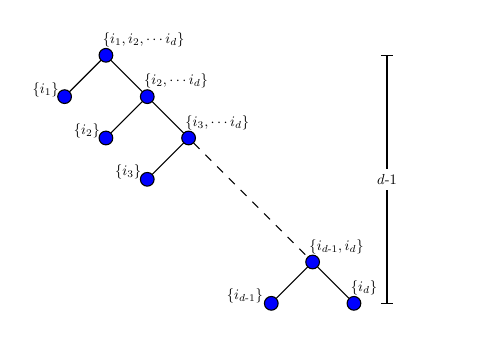
\begin{tikzpicture}[scale=0.525, every node/.style={transform shape}]
			%%\draw[fill=cyan] (0,0) circle (0.8cm);
			%%		\node [draw,circle]{r};
			%%		\tikzstyle{task}=[circle, draw, minimum size=10mm]
			%%		\node (d) at (0,0)[task, fill=babyblueeyes] {$D$};
			%%		\node (e) at (2.5,0)[task, fill=pastelviolet] {$E$};
			%%		\draw[thick, ->] (d.east) -- (e);
			%%		
			%%		\node (a) at (0,2)[task, fill=pastelyellow] {$A$};
			%%		\node (b) at (2.5,2.75)[task, fill=pastelgreen] {$B$};
			%%		\node (c) at (2.5,1.25)[task, fill=pastelred] {$C$};
			%%		
			%%		\draw[thick, ->] (a.east) -- (b);
			%%		\draw[thick, ->] (a.east) -- (c);
			\tikzstyle{taskc}=[circle, draw=black, minimum size=2mm, fill=blue]
			\tikzstyle{taskr}=[draw=none, minimum height=2mm, minimum width=5mm, anchor=south west, fill=none, text=black]
			%%
			\node (t01) at (0,0) [taskc]{};
			\node (t11) at (-1,-1) [taskc] {};
			\node (t12) at (1, -1) [taskc] {};
			\node (t21) at (0, -2) [taskc] {};
			\node (t22) at (2, -2) [taskc] {};
			\node (t31) at (1,-3) [taskc] {};
			\node (t52) at (5, -5) [taskc] {};
			\node (t61) at (4, -6) [taskc] {};
			\node (t62) at (6, -6) [taskc] {};
			
			\draw (t01) -- (t11);
			\draw (t01) -- (t12);
			\draw (t12) -- (t21);
			\draw (t12) -- (t22);
			\draw (t22) -- (t31);
			\draw [dashed] (t22) -- (t52);
			\draw (t52) -- (t61);
			\draw (t52) -- (t62);
			
			\draw (6.8, -6) -- (6.8, -3.25);
			\draw (6.8, -2.75) -- (6.8, 0);
			
			\draw (6.65, -6) -- (6.95, -6);
			\draw (6.65, -0) -- (6.95, 0);
			\node at (6.8, -3) {$d\text{-}1$};
			
			\node [above left=0mm and 2mm of t01.mid, taskr](l01) {$\{i_1,i_2,\cdots i_d\}$};
			\node [below left=2mm and 9mm of t11.mid, taskr](l11) {$\{i_1\}$};
			\node [above left=0mm and 2mm of t12.mid, taskr](l12) {$\{i_2,\cdots i_d\}$};
			\node [below left=2mm and 9mm of t21.mid, taskr](l21) {$\{i_2\}$};
			\node [above left=0mm and 2mm of t22.mid, taskr](l22) {$\{i_3,\cdots i_d\}$};
			\node [below left=2mm and 9mm of t31.mid, taskr](l31) {$\{i_3\}$};
			
			\node [above left=0mm and 2mm of t52.mid, taskr](l52) {$\{i_{d\text{-}1}, i_d\}$};
			\node [below left=2mm and 12mm of t61.mid, taskr](l61) {$\{i_{d\text{-}1}\}$};
			\node [above left=0mm and 2mm of t62.mid, taskr](l62) {$\{i_d\}$};
			
			\path (-0.1, -6.4) -- (8.5, -6.4); 
			\end{tikzpicture}
		} 
%%		\hfill
		\qquad\qquad
		\subfloat[Splitting of dimensions in PTT-decomposition.]{%
			\label{fig:ptt:workingtree}
			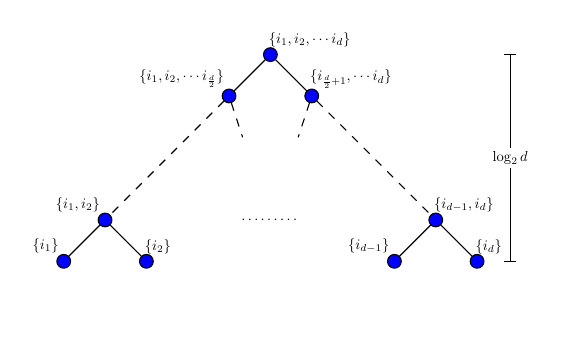
\begin{tikzpicture}[scale=0.525, every node/.style={transform shape}]
			
			\tikzstyle{taskc}=[circle, draw=black, minimum size=2mm, fill=blue]
			%%	\tikzstyle{taskr}=[draw=none, minimum height=2mm, minimum width=5mm, anchor=south west, fill=none, text=black]
			
			
			\node (t01) at (0,0) [taskc]{};
			\node (t11) at (-1,-1) [taskc] {};
			\node (t12) at (1, -1) [taskc] {};
			
			\node (tinter1) at (-0.5,-2) [taskc, draw=none, fill=none] {};
			\node (tinter2) at (0.5,-2) [taskc, draw=none, fill=none] {};
			
			\node (t41) at (-4,-4) [taskc] {};
			\node (t42) at (4,-4) [taskc] {};
			\node (t51) at (-5,-5) [taskc] {};
			\node (t52) at (-3,-5) [taskc] {};
			\node (t53) at (3,-5) [taskc] {};
			\node (t54) at (5,-5) [taskc] {};
			
			
			\draw (t01) -- (t11);
			\draw (t01) -- (t12);
			
			\draw [dashed] (t11) -- (tinter1.west);
			\draw [dashed] (t12) -- (tinter2.east);
			
			\draw [dashed] (t11) -- (t41);
			\draw [dashed] (t12) -- (t42);
			
			\path (t41) -- (t42) node [midway] {$\cdots\cdots\cdots$};
			
			\draw (t41) -- (t51);
			\draw (t41) -- (t52);
			
			\draw (t42) -- (t53);
			\draw (t42) -- (t54);
			
			
			\draw (5.8, -5) -- (5.8, -2.75);
			\draw (5.8, -2.25) -- (5.8, 0);
			
			\draw (5.65, -5) -- (5.95, -5);
			\draw (5.65, 0) -- (5.95, 0);
			\node at (5.8, -2.5) {$\log_2 d$};
			
			\node [above right] at (t01.160) {$\{i_1,i_2,\cdots i_d\}$};	
			
			\node [above left] at (t11.mid) {$\{i_1,i_2,\cdots i_\frac{d}{2}\}$};	
			\node [above right] at (t12.160) {$\{i_{\frac{d}{2}+1},\cdots i_d\}$};
			
			\node [above left] at (t41.mid) {$\{i_1,i_2\}$};
			\node [above right] at (t42.160) {$\{i_{d-1}, i_d\}$};
			
			\node [above left] at (t51.mid) {$\{i_1\}$};
			\node [above right] at (t52.160) {$\{i_2\}$};
			
			\node [above left] at (t53.mid) {$\{i_{d-1}\}$};
			\node [above right] at (t54.160) {$\{i_d\}$};
			
			
			\path (-0.1, -6.4) -- (2.5, -6.4); 
			%%		\path (-6.5, 0) -- (0,0);
			\end{tikzpicture}
		}
		%%		\includegraphics[scale=0.035]{./tt-ptt-decompositions.jpg}
		\caption{Splitting of dimensions in TT and PTT decompositions for a $d$-dimensional tensor. Each node shows a set of dimensions associated with it.~\label{fig:tt:ptt}}
	\end{center}
\end{figure*} 
Even if each step of the TT-decomposition can be parallelized, the separation of each dimension from the remaining ones is an intrinsically sequential process. This is reflected by the depth of the tree which is equal to one less than the number of dimensions of the tensor. From this figure, we also observe that we could achieve maximum parallelism if the tree is structured such that the width is full at each level. Based on this observation, we propose a parallel algorithm to compute TT-representation of a tensor and we call it Parallel Tensor Train (PTT) decomposition throughout the text. Designing communication optimal algorithms to compute TT-representation of a tensor is a part of our future work. Our PTT decomposition algorithm divides the tensor into two subtensors at each level. It exposes parallelism in a balanced binary tree shape and has maximum parallelism at the last level of the tree. Figure~\ref{fig:ptt:workingtree} shows the splitting of dimensions by this algorithm. We prove that the ranks of TT-representation computed by this algorithm are bounded by the ranks of unfolding matrices of the tensor. We also propose a parallel algorithm to compute approximation of a tensor in TT-representation. Our algorithm relies on a hierarchical partitioning of the dimensions of the tensor in a balanced binary tree shape and transmission of leading singular values of associated unfolding matrix from the parent to its children. We consider several approaches based on how leading singular values are transmitted in the tree and  evaluate them for different tensor sizes. Our results show that the approach which transmits leading singular values to both of its children performs better in practice. We also show that our algorithms transmit only $\mathcal{O}(\log^2 P\log d)$ number of messages along the critical path for a $d$-dimensional tensor on $P$ processors.

%%different tensor sizes. The main contributions of this paper are:
%%\begin{itemize}
%%	\item Propose a parallel algorithm PTT to compute TT-representation of a tensor
%%	\item Proof for bounded ranks of TT-representation obtained by PTT algorithm
%%	\item Different approaches to obtain approximation of a tensor in TT-format
%%	\item Numerous experiments to assess the effectiveness of our approaches for several low rank tensors and for tensors arising in quantum chemistry simulations. 
%%\end{itemize}

The rest of the paper is organized as follows. Section~\ref{sec:relatedWork} describes some popular tensor decompositions and their representations. In Section~\ref{sec:notationsAndTT}, we first present different notations required to express our algorithms, and then explain TT-representation and TT-decomposition algorithm. Parallel algorithms to compute decomposition and approximation of a tensor in TT-representation are presented in Sections~\ref{sec:tt_parallel} and~\ref{sec:approaches} respectively. In Section~\ref{sec:expResults}, we perform an assessment of our approximation algorithm for several low rank tensors. We finally propose conclusions and perspectives in Section~\ref{sec:conclusion}.

\section{Related Work}
\label{sec:relatedWork}
%0.5 page
Tensor decomposition was first introduced by \emph{Hitchcock} in 1927~\cite{hitchcock-1927}. This is now known as canonical polyadic (CP) decomposition (or CANDECOMP/PARAFAC).
It was rediscovered several times, mainly in psychometrics literature~\cite{redisover-candlecom-1,redisover-candlecom-2}.
It can be viewed as high order generalization of singular value decomposition (SVD). This represents a $d$-dimensional tensor \tensor{A} $\in \mathbb{R}^{n_1 \times \ldots \times n_d}$ with elements $\tensor{A}(i_1,\cdots,i_d)$ as, $\tensor{A}(i_1,\cdots,i_d) = \sum_{\alpha=1}^{r} U_1(i_1,\alpha) U_2(i_2,\alpha)\cdots U_d(i_d,\alpha)$. The minimum number of $r$ required to express \tensor{A} is called the canonical rank. The matrices $[U_k(i_k,\alpha)] \in \mathbb{R}^{n_i \times r}$, for $1 \leq k \leq d$, are called canonical factors. The number of entries in the decoupled representation is $\mathcal{O}(nrd)$, much less than the $\mathcal{O}(n^d)$ entries in the original tensor.
The most fascinating example of this decomposition in algorithmic complexity is Strassen matrix multiplication, which represents a $2 \times 2$ matrix multiplication as a decomposition of a $4\times4\times4$ tensor~\cite{strassen-matrix-multiplication}. 
This decomposition suffers from several drawbacks. Determining the canonical rank of a tensor is an NP-complete problem~\cite{canonical-rank-npcomplete} and $3$ or higher dimensional tensors can fail to have best approximations for a fixed canonical rank~\cite{tensor-rank-best-low-rank-approximation}. There are several algorithms to compute CP decomposition of a tensor for a fixed canonical rank~\cite{redisover-candlecom-1,ma2020accelerating,singh2020comparison}. The most popular one is alternating least squares. CP decomposition has also been considered for sparse tensors~\cite{candecomp-sparse}. It is difficult to apply conventional algorithms for large sparse tensors. Hence randomized algorithms are being employed to compute CP decomposition of these tensors~\cite{larsen2020practical}.

Matricized tensor times Khatri-Rao product (MTTKRP) is a key and time consuming operation in algorithms for computing CP decomposition of a tensor. There has been a lot of work in this context. Communication lower bounds for this operation have been established recently. Parallel and sequential algorithms that attain the lower bounds also have been presented~\cite{mttkrp-lowerbound}. Hypergraph based methods were proposed in~\cite{Kaya-SC-15} to balance the load and reduce the communication requirements of MTTKRP for distributed memory systems. A load balanced implementation of MTTKRP on GPUs is presented in~\cite{mttkrp-gpu}. An implementation of MTTKRP with hierarchical storage for sparse tensors has been presented recently in~\cite{hicoo}. 

%%There is not any deterministic procedure to find the best approximation of a tensor for a fixed canonical rank.

Another popular tensor decomposition is Tucker decomposition~\cite{tucker-decomposition}. This is also viewed as high order generalization of singular value decomposition. It decomposes a tensor into a set of matrices and a small core tensor. It is represented as, $\tensor{A}(i_1,\cdots,i_d) = \sum_{\alpha_1=1}^{r_1}\cdots\sum_{\alpha_d=1}^{r_d} g_{\alpha_1\cdots\alpha_d}U_1(i_1,\alpha_1)\cdots U_d(i_d, \alpha_d)$, where $\{ r_i \}_{1 \leq i \leq d}$ is a set of ranks. Tucker approximations can be computed by several SVDs for auxiliary matrices. The approximation computed by HOSVD algorithm increases the error at most by $\sqrt{d}$ with respect to the optimal error~\cite{hosvd-quasi-optimality}. For $r_1=r_2=\cdots =r_d=r$, Tucker approximations store $\mathcal{O}(ndr+r^d)$ entries. As the number of entries in this format is exponential in the number of dimensions, it is suitable for small dimensions, but not for large dimensions.

Tucker representation has further been improved 
in~\cite{h-tucker-Hackbusch_2009,h-tucker-Grasedyck}, and called 
Hierarchical Tucker (or H-Tucker). This is represented by a tree. Matrices of 
Tucker decomposition represent leaf nodes of this tree. Internal nodes 
correspond to the core tensor of the Tucker decomposition. Each internal 
node except root contains a $3$-dimensional tensor. Root node 
contains a matrix. The number of entries in this representation is 
$\mathcal{O}(ndr+dr^3)$.

As mentioned in the Introduction, TT-decomposition is a recently proposed tensor decomposition algorithm.
%%It is becoming very popular in several domains, e.g. quantum chemistry. 
We explain this algorithm in details in the next section. The TT-representation is known in the quantum chemistry community from a long time by the name of  matrix product states~\cite{mpsformat}. A communication efficient parallel algorithm to perform rounding in TT-format has recently been proposed~\cite{ballard2019}. 

\section{Notations \& TT-Representation}
\label{sec:notationsAndTT}
% 0.5 page
%%\begin{itemize}
%%%%	\item Tensor train decomposition
%%	\item Complexity and its analysis
%%\end{itemize}
\noindent Let $\tensor{A}(i_1,i_2,\cdots, i_d)$ denote the elements of a $d$-dimensional tensor \tensor{A} $\in \mathbb{R}^{n_1 \times n_2 \times \cdots \times n_d}$. We use bold letters to denote tensors. The $k$-th unfolding matrix of tensor \tensor{A} is represented by $A_k$.

$\qquad\qquad A_k = [A_k(i_1, i_2,\cdots, i_k; i_{k+1},\cdots ,i_d)]$

%%\begin{align*}
%%\qquad\qquad A_k = [A_k(i_1, i_2,\cdots, i_k; i_{k+1},\cdots ,i_d)]
%%\end{align*}
\noindent The first $k$ indices represent the rows of $A_k$ and the last $d$-$k$ the columns of $A_k$. The size of this matrix is $(\prod_{l=1}^{k}n_l)\times(\prod_{l=k+1}^{d}n_l)$. The rank of this matrix is denoted by $r_k$. Let ($r_1, r_2,\cdots, r_{d-1}$) denote the ranks of unfolding matrices of tensor \tensor{A}.

Let $A(i;j)$ denote the element of $i$th row and $j$th column of a matrix $A$. $i$ and $j$ can be set of indices. For example, row and column indices of element $A_k(i_1, i_2,\cdots, i_k; i_{k+1},\cdots ,i_d)$ are the entries corresponding to $(i_1, i_2,\cdots, i_k)$ and $(i_{k+1},\cdots ,i_d)$ in rows and columns of $A_k$ respectively.

Let $||\tensor{A}||_F$ denote the frobenius norm of a $d$-dimensional tensor \tensor{A} and it is defined as, $||\tensor{A}||_F=$ $\sqrt{\sum_{i_1, i_2, \cdots, i_d}A(i_1,i_2,\cdots, i_d)^2 }$. $||A||_2$ and $||A||_F$ denote the spectral norm and the frobenius norm of a matrix $A$ and they are defined as, $||A||_2 = $ \textit{maximum singular value of} $A$ and $||A||_F = \sqrt{\sum_{i,j} A(i;j)^2}$. Let $tr(A)$ denote the trace of a square matrix $A$ and it is computed as, $tr(A) = \sum_i A(i;i)$.

\subsection{TT-Representation}
An efficient representation of a tensor with small number of variables provides opportunities to work with high dimensional tensors. TT-representation is a popular way to represent such tensors with few number of variables, as discussed in~\cite{tt}. It represents a $d$-dimensional tensor with $2$ matrices and $d$-$2$ $3$-dimensional tensors. These are called cores of the TT-representation.


In TT-representation, a $d$-dimensional tensor $\tensor{A}$ $\in$ $\mathbb{R}^{n_1 \times n_2 \times \cdots \times n_d}$ is represented with cores $\tensor{G}_k$ of size $r_{k-1}\times n_k\times r_k$, $k=1,2,\cdots d$, $r_0=r_d=1$ and its elements satisfy the following expression:
{\small\begin{align*}
	\tensor{A}(i_1,\cdots ,i_d) 
	&= \sum_{\alpha_0 = 1}^{r_0} \cdots \sum_{\alpha_d = 1}^{r_d} \tensor{G}_1(\alpha_0, i_1, \alpha_1) \cdots \tensor{G}_d(\alpha_{d-1}, i_d, \alpha_d)\\
	&= \sum_{\alpha_1 = 1}^{r_1} \cdots \sum_{\alpha_{d-1} = 1}^{r_{d-1}} \tensor{G}_1(1, i_1, \alpha_1) \cdots \tensor{G}_d(\alpha_{d-1}, i_d, 1)
	\end{align*}}

Here $\tensor{G}_k(\alpha_{k-1}, i_k, \alpha_k)$ are the elements of $\tensor{G}_k$. Since $r_0=r_d=1$, $\tensor{G}_1$ and $\tensor{G}_d$ cores are matrices. The other cores are $3$-dimensional tensors. First and last cores are matrices, we still use bold letters to represent all cores. For $n_1=n_2=\cdots=n_d=n$ and $r_1=r_2=\cdots=r_{d-1}=r$, the number of entries in this representation is $\mathcal{O}(ndr^2)$.


\begin{figure}[htb]
	\begin{center}
		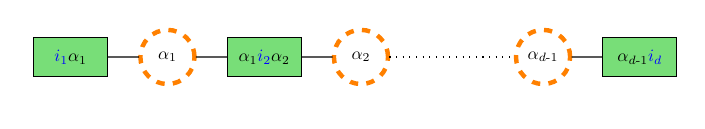
\begin{tikzpicture}[scale=0.625, every node/.style={transform shape}]
		%%\draw[fill=cyan] (0,0) circle (0.8cm);
		\tikzstyle{taskc}=[circle, draw=orange, minimum size=11mm, fill=white, dashed, ultra thick]
		\tikzstyle{taskr}=[draw=black, minimum height=8mm, minimum width=15mm, anchor=south west, fill=pastelgreen, text=black]
		
		\node(t1) at (0,0) {};
		\node [above right=0cm and 0cm of t1.mid,taskr](T1) {$\textcolor{blue}{i_1}\alpha_1$};
		\node [above right=0cm and 0.8cm of T1.south east, taskc](C1) {$\alpha_1$};
		\node [above right=0cm and 0.8cm of C1.south east, taskr](T2) {$\alpha_1\textcolor{blue}{i_2}\alpha_2$};
		\node [above right=0cm and 0.8cm of T2.south east, taskc](C2) {$\alpha_2$};
		
		\node [above right=0cm and 4.5cm of T2.south east, taskc](Cd) {$\alpha_{d\text{-}1}$};
		\node [above right=0cm and 0.8cm of Cd.south east, taskr](Td) {$\alpha_{d\text{-}1}\textcolor{blue}{i_d}$};
		%%\node (d) at (0,0)[taskc, fill=babyblueeyes] {$D$};
		%%\node (e) at (2.5,0)[taskc, fill=pastelviolet] {$E$};
		%%\draw[thick, ->] (d.east) -- (e);
		%%
		%%\node (a) at (0,2)[taskr, minimum width=3cm, fill=pastelyellow, text=blue, thick, draw=blue] {$A_b + C_d$};
		%%\node (b) at (2.5,2.75)[taskc, fill=pastelgreen] {$B$};
		%%\node (c) at (2.5,1.25)[taskc, fill=pastelred] {$C$};
		%%
		%%\draw[thick, ->] (a.east) -- (b);
		%%\draw[thick, ->] (a.east) -- (c);
		\draw (T1.east)--(C1.west);
		\draw (C1.east)--(T2.west);
		\draw (T2.east)--(C2.west);
		\draw [dotted] (C2.east)--(Cd.west);
		\draw (Cd.east)--(Td.west);
		
		\path (-0.1, -0.4) -- (2.5, -0.4); 
		%%\path (-0.1, -0.8) -- (2.5, -0.8); 
		\end{tikzpicture}
		%%		\includegraphics[scale=0.05]{./chaintt.jpg}
		\caption{Chain diagram of TT-representation.\label{fig:ttrainchain}}
	\end{center}
\end{figure}
Figure~\ref{fig:ttrainchain} exhibits that the above expression can also be represented graphically by a linear chain where sum over circle nodes (indices $\alpha_k$) are assumed to compute an entry of the tensor. This figure looks like a train, hence the tensor train name is used for the representation. 
\begin{figure}[!b]
	\begin{center}	
		\includegraphics[scale=0.5]{./ttentry.eps}
		\caption{TT-representation of a $d$-dimensional tensor $\tensor{A}$ $\in$ $\mathbb{R}^{n_1 \times n_2 \times \cdots \times n_d}$. An entry of the tensor is computed by multiplying corresponding matrix (or row/column) of each core.\label{fig:ttdiagram}}
	\end{center}
\end{figure}

Figure~\ref{fig:ttdiagram} also shows how an entry of a tensor can be computed with the cores of TT-representation. With a slight abuse of notation, $\tensor{G}_k(i_k)$ denotes the $i_k$th slice of $k$th core of TT-representation.


\subsection{TT-Decomposition}
As mentioned earlier, the TT-Decomposition algorithm has been proposed in~\cite{tt} to compute TT-representation of a tensor. Here we present the main idea of the algorithm. Let \tensor{A} $\in \mathbb{R}^{n_1 \times n_2 \times \cdots \times n_d}$ be a $d$-dimensional tensor. The algorithm operates in $d$-$1$ steps. In each step, one dimension of the tensor is decoupled from the remaining dimensions using SVD. In the first step, \tensor{A} is represented as a matrix of size $n_1$ $\times$ $n_2 n_3 \cdots n_d$ and SVD is computed for this matrix. The left singular vectors corresponding to nonzero singular values are the first core of TT-representation. In the second step, interaction with the first core and the second dimension are represented as rows of the matrix while other dimensions $n_3\cdots n_d$ represent the columns. Again SVD is computed for this matrix and left singular vectors are rearranged to obtain the second core of TT-representation. This process is repeated for $d$-$1$ steps. Hence $d$-$1$ cores are obtained by this process. Remaining matrix, which represents the interaction with the ($d$-$1$)th core and $n_d$, constitutes the last core of the representation. This algorithm produces cores $\tensor{G}_k(\alpha_{k-1}, n_k, \alpha_k) _{1\le k\le d}$ and also ensures that $\alpha_k \le r_k$. We refer the reader to the original paper for more details about this algorithm. 


The separation of each dimension from the remaining ones is a sequential process in TT-decomposition. Most modern computing platforms are composed of several number of nodes and cores. Hence running a sequential process on these platforms may result in poor utilization of resources. In the next section, we propose a parallel algorithm to obtain TT-representation of a tensor.

\section{Parallel TT Decomposition}
\label{sec:tt_parallel}
% 2.5 pages
%%\begin{itemize}
%%%%	\item Different notations
%%%%	\item Parallel Tensor train algorithm and its proof
%%	\item Working principle with a matrix diagram and its reshape property
%%	\item Its generalization idea that we can break it from anywhere
%%\end{itemize}
The original indices of a tensor are called external indices, while the indices obtained due to SVD are called internal indices. $nEI(\tensor{A})$ denotes the number of external indices of a tensor \tensor{A}. A tensor with elements $\tensor{A}(\alpha, i_1, i_2, i_3, \beta)$ has $3$ external and $2$ internal indices. We also extend the definition of unfolding matrix to take internal indices into account. The $k$-th unfolding of tensor \tensor{A}, whose elements are $\tensor{A}(\alpha, i_1, i_2, \cdots,i_k, i_{k+1}, \cdots, \beta)$, is represented as, $ A_k = [A_k(\alpha, i_1, i_2, \cdots, i_k; i_{k+1}\cdots, \beta)]$. Here we consider all indices from the beginning to $i_{k}$ as the rows of $A_k$ and the remaining indices as the columns of $A_k$.


Let \textbf{Tensor}($A_l$) convert an unfolding matrix $A_l$ to its tensor form. For example, if $A_l(\alpha, i_1,\cdots,i_l;i_{l+1}\cdots,i_m, \beta)$ represent the elements of an unfolding matrix $A_l$ then \textbf{Tensor}($A_l$) produces a tensor \tensor{A} with elements $\tensor{A}(\alpha, i_1,\cdots, i_l, i_{l+1},\cdots, i_m, \beta)$.
\begin{algorithm}[htb]
	\caption{\label{alg:tt_parallel}PTT-decomposition (parallel Tensor Train Decomposition)}
	\begin{algorithmic}[1]
		\REQUIRE $d$-dimensional tensor \tensor{A} and ranks ($r_1, r_2,\cdots r_{d-1}$) 
		\ENSURE Cores $\tensor{G}_k(\alpha_{k-1}, n_k, \alpha_k) _{1\le k\le d}$ of the TT-representation with $\alpha_k \le r_k$ and $\alpha_0 = \alpha_d=1$
		\IF{$nEI(\tensor{A})> $$1$} 
		\STATE Find the middle external index $k$
		\STATE Compute unfolding matrix $A_k$ 
		\STATE Compute SVD: $A_k = U \Sigma V^T$
		\STATE Compute rank of $\Sigma$, $\alpha_k=$ rank($\Sigma$)
		\STATE Select diagonal matrices $X_k$, $S_k$ and $Y_k$ such that $X_kS_kY_k = \Sigma(1:\alpha_k; 1:\alpha_k)$\label{alg:line:xsy}
		%%		\STATE // first $\alpha_k$ columns of $U$
		\STATE $\tensor{A}$$_{left}$ = \textbf{Tensor}($U(;1:\alpha_k)X_k$)
		\STATE list1 = PTT-decomposition($\tensor{A}$$_{left}$, ($r_1,\cdots r_{k-1},\alpha_k$) )
		\STATE $\tensor{A}$$_{right}$ = \textbf{Tensor}($Y_kV^T(1:\alpha_k;)$)
		\STATE list2= PTT-decomposition($\tensor{A}$$_{right}$,($\alpha_k, r_{k+1},\cdots r_{d-1}$))
		\RETURN \{list1, list2\}
		\ELSE 
		\STATE Find the external index $k$
		\IF {$k$ is the last index of \tensor{A}} 
		\STATE $\alpha_k = 1$
		%%		\ENDIF
		\ELSIF {$k$ is the first index of \tensor{A}}
		\STATE $\alpha_{k\text{-}1} = 1$
		\STATE $\tensor{A}(i_k, \beta)$ = $\sum_{\beta=1}^{\alpha_k} \tensor{A}(i_k, \beta)S_k(\beta;\beta)$ \label{alg:ptt:firstcore}
		\ELSE
		\STATE $ \tensor{A}(\gamma, i_k, \beta)$ = $\sum_{\beta=1}^{\alpha_k} \tensor{A}(\gamma, i_k, \beta)S_k(\beta;\beta)$\label{alg:ptt:otherthanfirstcore}
		\ENDIF
		\STATE $\tensor{G}_k$ = $ \tensor{A}$
		\STATE return $\tensor{G}_k$
		\ENDIF
	\end{algorithmic}
\end{algorithm} 

We present a parallel algorithm to compute TT-representation of a tensor in Algorithm~\ref{alg:tt_parallel}. It is possible to work directly with unfolding matrices, however for the ease of presentation, intermediate unfolding matrices are converted to tensors. We can also note that selection of $X_k$, $S_k$ and $Y_k$ is not specified in line number~\ref{alg:line:xsy}. Our proof applies no matter how these are chosen. However, the practical performance of the approximation algorithm, which is based on this algorithm, depends on the selection of these matrices. In Section~\ref{sec:expResults}, we compare three options: i) $X_k=S_k=I$, $Y_k = \Sigma(1:\alpha_k; 1:\alpha_k)$ ii) $X_k = Y_k = \Sigma(1:\alpha_k; 1:\alpha_k)^{1/2}$, $S_k = I$ iii) $X_k = Y_k = \Sigma(1:\alpha_k; 1:\alpha_k)$, $S_k = \Sigma(1:\alpha_k; 1:\alpha_k)^{-1} $. In most cases, third option is often the better choice.

In PTT-decomposition algorithm, if the input tensor \tensor{A} has more than one external index then first we compute the middle external index $k$. After that, we compute the rank $\alpha_k$ and the SVD of the unfolding matrix $A_k$. Three diagonal matrices $X_k$, $S_k$ and $Y_k$ are chosen such that their product corresponds to the matrix obtained by selecting leading $\alpha_k$ rows and columns of the singular value matrix. Selection of the diagonal matrices is related to how singular values will be transferred in recursive calls. Now, a matrix containing leading $\alpha_k$ left singular vectors is multiplied by $X_k$. The result is converted in tensor format and PTT-decomposition algorithm is called for this subtensor. Similarly, $Y_k$ is multiplied by a matrix which contains the transpose of leading $\alpha_k$ right singular vectors, and again PTT-decomposition algorithm is called with the tensor format of the result. When the call for both functions returns, we receive cores of TT-representations of both subtensors. We combine them and this constitutes a TT-representation of \tensor{A}.
%% We return the cores of this representation.

Now we consider the case when number of external indices in the tensor is $1$. If the external index $k$ is the last index then we want to compute the last core of the TT-representation. Hence we simply assign the current tensor to the last core and this is returned to the caller. When the external index corresponds to the first or last index of the tensor, we set $\alpha_0$ or $\alpha_d$ appropriately for the core. For the correctness, now the input tensor is multiplied with the diagonal matrix $S_k$, and the result is assigned to the $k$th core of the TT-representation. In the end, this core is returned to the caller. 

\begin{figure}[!htb]
	\begin{center}
		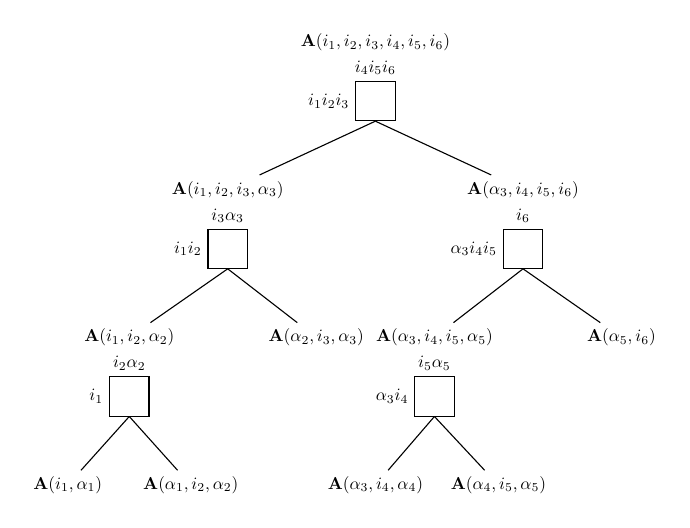
\begin{tikzpicture}[scale=0.625, every node/.style={transform shape}]
		\tikzstyle{taskr}=[draw=black, minimum height=8mm, minimum width=8mm, fill=none, text=black]
		%%	anchor=south west,
		\node (t10) at (0,1.2) {$\tensor{A}(i_1,i_2,i_3,i_4,i_5,i_6)$};	
		\node (b01) at (0,0) [taskr]{};
		\node [above] at (b01.north) {$i_4i_5i_6$};
		\node [left] at (b01.west) {$i_1i_2i_3$};		
		
		\node (t11) at (-3,-1.8) {$\tensor{A}(i_1,i_2,i_3,\alpha_3)$};
		\node (t12) at (3,-1.8) {$\tensor{A}(\alpha_3, i_4, i_5, i_6)$};
		
		\draw (b01.south) -- (t11);	
		\draw (b01.south) -- (t12);
		
		\node (b11) at (-3,-3) [taskr]{};
		\node (b12) at (3,-3) [taskr]{};
		
		\node [above] at (b11.north) {$i_3\alpha_3$};
		\node [left] at (b11.west) {$i_1i_2$};
		
		\node [above] at (b12.north) {$i_6$};
		\node [left] at (b12.west) {$\alpha_3i_4i_5$};
		
		\node (t21) at (-5, -4.8) {$\tensor{A}(i_1,i_2,\alpha_2)$};
		\node (t22) at (-1.2, -4.8) {$\tensor{A}(\alpha_2, i_3,\alpha_3)$};
		
		\node (t23) at (1.2, -4.8) {$\tensor{A}(\alpha_3,i_4,i_5,\alpha_5)$};
		\node (t24) at (5, -4.8) {$\tensor{A}(\alpha_5, i_6)$};
		
		\draw (b11.south) -- (t21);
		\draw (b11.south) -- (t22);
		
		\draw (b12.south) -- (t23);
		\draw (b12.south) -- (t24);		
		
		\node (b21) at (-5,-6) [taskr]{};
		\node [above] at (b21.north) {$i_2\alpha_2$};
		\node [left] at (b21.west) {$i_1$};
		
		\node (b22) at (1.2,-6) [taskr]{};
		\node [above] at (b22.north) {$i_5\alpha_5$};
		\node [left] at (b22.west) {$\alpha_3i_4$};
		
		\node (t31) at (-6.25, -7.8) {$\tensor{A}(i_1,\alpha_1)$};
		\node (t32) at (-3.75, -7.8) {$\tensor{A}(\alpha_1,i_2,\alpha_2)$};
		
		\draw (b21.south) -- (t31);
		\draw (b21.south) -- (t32);
		
		\node (t33) at (0, -7.8) {$\tensor{A}(\alpha_3,i_4,\alpha_4)$};
		\node (t34) at (2.5, -7.8) {$\tensor{A}(\alpha_4,i_5,\alpha_5)$};
		
		\draw (b22.south) -- (t33);
		\draw (b22.south) -- (t34);
		
		\end{tikzpicture}
	\end{center}
	\caption{Diagramatic representation of unfolding matrices at all non-leaf nodes for a $6$-dimensional tensor by Algorithm~\ref{alg:tt_parallel}.\label{fig:ptt:reshaping}}
\end{figure}

PTT-decomposition algorithm returns the cores of a TT presentation for \tensor{A}. This algorithm exposes parallelism in a binary tree shape. It achieves maximum $\mathcal{O}(d)$-level of parallelism at the last level of the tree.

Figure~\ref{fig:ptt:reshaping} illustrates the working tree of Algorithm~\ref{alg:tt_parallel} for a $6$-dimensional tensor. It shows a tensor at each node in its index form. It also displays unfolding matrices for non-leaf nodes. Cores of the TT-representation are assigned at leaf nodes after multiplying the subtensors with corresponding $S_k$ matrices (Lines~\ref{alg:ptt:firstcore} and~\ref{alg:ptt:otherthanfirstcore} of Algorithm~\ref{alg:tt_parallel}). 

We can notice that working tree of our algorithm is similar to Hierarchical Tucker~\cite{h-tucker-Grasedyck}. However, intrinsic details of both algorithms are quite different. In our algorithm, cores of the TT-representation are assigned at leaf nodes. While in Hierarchical Tucker algorithms, compressed representation is stored in a tree format. Leaf nodes correspond to factor matrices of Tucker decomposition and each internal node stores a $3$-dimensional tensor or a matrix. All internal nodes combined together correspond to the core tensor of Tucker decomposition.

The proof on the bound of TT ranks obtained by Algorithm~\ref{alg:tt_parallel} is described in the following theorem.

\begin{theorem}
	If for each unfolding $A_k$ of a $d$-dimensional tensor \tensor{A}, $rank(A_k)=r_k$, then Algorithm~\ref{alg:tt_parallel} produces a TT-representation with ranks not higher than $r_k$.
\end{theorem}
\begin{proof}
	Let us consider the unfolding matrix $A_k$ of a $d$-dimensional tensor \tensor{A}$\in \mathbb{R}^{n_1 \times \ldots \times n_d}$. The SVD of $A_k$ is represented as, $A_k = U \Sigma V^T$. The rank of the unfolding matrix is $r_k$; hence it can be written as:
	\begin{align*}
	&A_k(i_1,\cdots,i_k;i_{k+1},\cdots, i_d)\\
	&\qquad= \sum_{\alpha=1}^{r_k} U(i_1,\cdots,i_k; \alpha)\Sigma(\alpha; \alpha)V^T(\alpha;i_{k+1},\cdots, i_d)\\
	&\qquad= \sum_{\alpha=1}^{r_k} U(i_1,\cdots,i_k; \alpha)X(\alpha; \alpha)S(\alpha; \alpha)Y(\alpha; \alpha) V^T(\alpha;i_{k+1},\cdots, i_d)\\
	&\qquad= \sum_{\alpha=1}^{r_k} B(i_1,\cdots,i_k; \alpha)S(\alpha; \alpha)C(\alpha;i_{k+1},\cdots, i_d).
	\end{align*}
	In matrix form we obtain,
	\begin{align*}
	A_k = BSC,\quad\ \ &\\
	\quad B = A_k C^{-1}S^{-1} &= A_kZ, \\
	\quad C = S^{-1}B^{-1}A_k &= WA_k,
	%%	\quad B = A_k (C^T)^{-1}S^{-1} &= A_kZ\\
	%%	\quad C = A_k^T (B^T)^{-1}S^{-1} &= A_k^T W
	\end{align*}
	\noindent or in the index form,
	{\small\begin{align*}
		&B(i_1,\cdots, i_k; \alpha) = \sum_{i_{k+1}=1}^{n_{k+1}}\cdots\sum_{i_d=1}^{n_d} \tensor{A}(i_1, \cdots, i_d) Z(i_{k+1},\cdots, i_d;\alpha), \\
		&C(\alpha; i_{k+1},\cdots, i_d) = \sum_{i_1=1}^{n_1} \cdots \sum_{i_k=k}^{n_k} \tensor{A}(i_1, \cdots, i_d) W(\alpha;i_1,i_2,\cdots, i_k).
		\end{align*}}
	
	\noindent $B$ and $C$ can be treated as $k+1$ and $d$-$k+1$ dimensional tensors \tensor{B} and \tensor{C} respectively. Now we consider unfolding matrices $B_1$, $\cdots$, $B_{k-1}$ and $C_{k+1}$, $\cdots$, $C_{d-1}$ of \tensor{B} and \tensor{C}. We will show that rank($B_{k'}$)$ \le r_{k'}$ $_{1\le k' \le k-1}$ and rank($C_{k'}$)$\le r_{k'}$ $_{k+1\le k' \le d-1}$.
	
	\noindent The rank of $A_{k'}$ is $r_{k'}$. Therefore, $\tensor{A}$ can be represented as,
	\begin{align*}
	\tensor{A}(i_1, \cdots, i_d) &= \sum_{\beta=1}^{r_{k'}} F(i_1,\cdots ,i_{k'}; \beta) G(\beta; i_{k'+1},\cdots, i_d)
	\end{align*}
	\noindent Now,
	
	\noindent $B_{k'} = [B_{k'}(i_1, \cdots, i_{k'}; i_{k'+1},\cdots,i_k, \alpha)]$
	\begin{align*}
	&B_{k'}(i_1, \cdots, i_{k'}; i_{k'+1},\cdots,i_k, \alpha)\\
	&\quad= \sum_{i_{k+1}=1}^{n_{k+1}}\cdots\sum_{i_d=1}^{n_d} \tensor{A}(i_1, \cdots, i_d)Z(i_{k+1},\cdots, i_d;\alpha)\\
	&\quad= \sum_{\beta=1}^{r_{k'}} \sum_{i_{k+1}=1}^{n_{k+1}}\cdots\sum_{i_d=1}^{n_d} F(i_1,\cdots ,i_{k'}; \beta) G(\beta; i_{k'+1},\cdots, i_d)\\
	& \qquad\qquad\qquad\qquad\qquad\qquad\qquad\qquad\quad Z(i_{k+1}, \cdots, i_d;\alpha)\\
%%	 Z(i_{k+1}, \cdots, i_d;\alpha)\\
	&\quad= \sum_{\beta=1}^{r_{k'}} F(i_1,i_2,\cdots ,i_{k'}; \beta) H(\beta; i_{k'+1},\cdots, i_k, \alpha).
	\end{align*}
	\noindent where,
	\begin{align*}
	&H(\beta;i_{k'+1},\cdots, i_k, \alpha)\\ 
	&\qquad= \sum_{i_{k+1}=1}^{n_{k+1}}\cdots\sum_{i_d=1}^{n_d} G(\beta; i_{k'+1},\cdots, i_d) Z(i_{k+1},\cdots, i_d;\alpha).
	\end{align*}
	\noindent Row and column indices of $B_{k'}$ are now separated. Hence rank($B_{k'}$)$ \le r_{k'}$.
	
	\medskip
	\noindent Similarly for $C_{k'}$,
	
	\noindent $C_{k'}= [C_{k'}(\alpha, i_{k+1}, \cdots, i_{k'}; i_{k'+1},\cdots, i_d)]$
	\begin{align*}
	&C_{k'}(\alpha, i_{k+1}, \cdots, i_{k'}; i_{k'+1},\cdots, i_d)\\
	&\quad= \sum_{i_1=1}^{n_1} \cdots \sum_{i_k=k}^{n_k} \tensor{A}(i_1, i_2, \cdots, i_d) W(\alpha; i_1,i_2,\cdots, i_k)\\
	&\quad= \sum_{\beta=1}^{r_{k'}} \sum_{i_1=1}^{n_1} \cdots \sum_{i_k=k}^{n_k} F(i_1,i_2,\cdots ,i_{k'}; \beta) G(\beta; i_{k'+1},\cdots, i_d)\\
	&\qquad\quad\qquad\qquad\qquad\qquad\qquad\qquad\qquad W(\alpha; i_1,i_2,\cdots, i_k)\\
%%	 W(\alpha; i_1,i_2,\cdots, i_k)\\ 
	&\quad= \sum_{\beta=1}^{r_{k'}} M(\alpha, i_{k+1}, \cdots, i_{k'}; \beta) G(\beta; i_{k'+1},\cdots, i_d).
	\end{align*}	
	\noindent where,
	\begin{align*}
	&M(\alpha, i_{k+1}, \cdots, i_{k'}; \beta)\\ 
	&\qquad= \sum_{i_1=1}^{n_1} \cdots \sum_{i_k=k}^{n_k} F(i_1,i_2,\cdots ,i_{k'}; \beta) W(\alpha; i_1,i_2,\cdots, i_k).
	\end{align*}
	\noindent Here also row and column indices of $C_{k'}$ are separated. Hence rank($C_{k'}$)$ \le r_{k'}$.
	
	\noindent As the above proof holds for each recursive partition, hence  ranks of the TT-representation produced by Algorithm~\ref{alg:tt_parallel} are bounded by $r_k$. This completes the proof.
\end{proof}

\indent The above proof is independent of from which index we split the tensor into two subtensors. However in Algorithm~\ref{alg:tt_parallel}, we split the tensor from the middle external index.


\section{Approximations of the Parallel TT Decomposition}
\label{sec:approaches}
% 1 page
%%\begin{itemize}
%%	\item Our approaches
%%	\item different performance metrics
%%\end{itemize}
%%Tensor decompositions are often approximated with a controllable global error to cope with noise and numerical instability. 
Tensor decompositions are often approximated to cope with large amounts of data while controlling the loss of accuracy. In practical computations, rank-$r_k$ approximation of a tensor or an approximated tensor with certain accuracy is desired. Algorithm~\ref{alg:tt_parallel} can be used to compute rank-$r_k$ approximation of a tensor instead of exact low-rank decomposition. However we are yet to claim any optimality on its approximation and it is a part of our future work.

We modify Algorithm~\ref{alg:tt_parallel} to compute an approximated tensor in TT-representation that is less than or close to the prescribed accuracy, and present it in Algorithm~\ref{alg:tt_parallel_approx}.

\begin{algorithm}[htb]
	\caption{\label{alg:tt_parallel_approx}PTT-approx (parallel Tensor Train approximation)}
	\begin{algorithmic}[1]
		\REQUIRE $d$-dimensional tensor \tensor{A} and expected accuracy $\epsilon$ 
		\ENSURE Cores $\tensor{G}_k(\alpha_{k-1}, n_k, \alpha_k) _{1\le k\le d}$ of the approximated tensor \tensor{B} in TT-representation such that $||\tensor{A}-\tensor{B}||_F$ is close to or less than $\epsilon$
		\IF{$nEI(\tensor{A})> $$1$} 
		\STATE Find the middle external index $k$
		\STATE Compute unfolding matrix $A_k$ 
		\STATE Compute SVD: $A_k = U \Sigma V^T$
		\STATE Compute truncation accuracy $\Delta$
		\STATE Compute $\alpha_k$ such that $A_k = U(;1:\alpha_k) \Sigma(1:\alpha_k; 1:\alpha_k) V^T(1:\alpha_k;) + E_k$ and $||E_K||_F \le \Delta$
		\STATE Select diagonal matrices $X_k$, $S_k$ and $Y_k$ such that $X_kS_kY_k = \Sigma(1:\alpha_k; 1:\alpha_k)$
		\STATE $\tensor{A}$$_{left}$ = \textbf{Tensor}($U(;1:\alpha_k)X_k$)
		\STATE list1 = PTT-approx($\tensor{A}$$_{left}$, $\epsilon_1$)
		\STATE $\tensor{A}$$_{right}$ = \textbf{Tensor}($Y_kV^T(1:\alpha_k;)$)
		\STATE list2 = PTT-approx($\tensor{A}$$_{right}$, $\epsilon_2$)
		\RETURN \{list1, list2\}
		\ELSE 
		\STATE Find the external index $k$
		\IF {$k$ is the last index of \tensor{A}} 
		\STATE $\alpha_k = 1$
		%%		\ENDIF
		\ELSIF {$k$ is the first index of \tensor{A}}
		\STATE $\alpha_{k\text{-}1} = 1$
		\STATE $\tensor{A}(i_k, \beta)$ = $\sum_{\beta=1}^{\alpha_k} \tensor{A}(i_k, \beta)S_k(\beta;\beta)$
		\ELSE
		\STATE $ \tensor{A}(\gamma, i_k, \beta)$ = $\sum_{\beta=1}^{\alpha_k} \tensor{A}(\gamma, i_k, \beta)S_k(\beta;\beta)$
		\ENDIF
		\STATE $\tensor{G}_k$ = $ \tensor{A}$
		\STATE return $\tensor{G}_k$
		\ENDIF
	\end{algorithmic}
\end{algorithm}

Expected accuracy is also an input to Algorithm~\ref{alg:tt_parallel_approx}. $\alpha_k$ is selected based on truncation accuracy $\Delta$ of the unfolding matrix. Approximations of left and right subtensors are called with expected accuracies of $\epsilon_1$ and $\epsilon_2$. Values of $\delta$, $\epsilon_1$ and $\epsilon_2$ in Algorithm~\ref{alg:tt_parallel_approx} depend on the truncation accuracy of the unfolding matrix and how leading singular values are passed to both subtensors (depend on selection of diagonal matrices $X_k$, $Y_k$ and $S_K$). We show in next subsection how the product of approximated matrices impacts the accuracy of the result when applied with SVD truncation. Based on the expression of the next subsection, we compute $\epsilon_1$ and $\epsilon_2$ for different choices of $X_k$, $Y_k$ and $S_K$ in Section~\ref{sec:approaches:all}. 

\subsection{Frobenius Error with Product of Approximated Matrices}
\label{sec:approaches:approxproduct}

The SVD of a real matrix $A$ is written as, $A=U\Sigma V^T$. This decomposition can also be written as,
\begin{align*}
A&=(U_1 U_2)\begin{pmatrix}
\Sigma_1 & 0\\
0 & \Sigma_2
\end{pmatrix}(V_1 V_2)^T = U_1\Sigma_1 V_1^T + U_2 \Sigma_2 V_2^T\\
&= U_1\Sigma_1 V_1^T + E_A = BSC + E_A.
\end{align*}

\noindent Here $B = U_1 X$, $C=YV_1^T$ and $XSY = \Sigma_1$. Matrices $B$ and $C$ are approximated by $\hat{B}$ and $\hat{C}$, i.e., $B = \hat{B} + E_B$ and $C = \hat{C} + E_C$. $X$, $Y$ and $S$ are diagonal matrices. $E_A$, $E_B$ and $E_C$ represent error matrices corresponding to low-rank approximations of $A$, $B$ and $C$. We are interested to find an expression for $||A - \hat{B} S \hat{C}||_F$ in terms of $||E_A||_F$, $||E_B||_F$ and $||E_C||_F$. We have,
\begin{align*}
A - \hat{B} S \hat{C} &= A - (B-E_B)S(C-E_C)\\
&= A - BSC + BSE_C + E_BSC - E_BSE_C\\
&= E_A + BSE_C + E_BSC - E_BSE_C
\end{align*}
Now we take square of Frobenius norm on both sides,
\begin{align*}
&||A - \hat{B} S \hat{C}||_F^2 \\ 
&\qquad= ||E_A + BSE_C + E_BSC - E_BSE_C||_F^2 \\
&\qquad= ||E_A||_F^2 + ||BSE_C||_F^2 + ||E_BSC||_F^2 + ||E_BSE_C||_F^2 \\
&\qquad\quad + 2\boldsymbol{<}E_A, BSE_C\boldsymbol{>}_F + 2<E_A, E_BSC>_F \\
&\qquad\quad -2 <E_A, E_BSE_C>_F + 2 <BSE_C, E_BSC>_F \\
&\qquad\quad -2 <BSE_C, E_BSE_C>_F - 2<E_BSC, E_BSE_C>_F.
\end{align*}

\noindent Here $<P, Q>_F$ denotes frobenius inner product of matrices $P$ and $Q$, and it is defined as: $<P, Q>_F = tr(P^TQ) = tr(PQ^T)$. As $U$ and $V$ are othogonal matrices obtained from the SVD of $A$, we obtain the following expressions:
\begin{align*}
U_1^TU_2 = 0 & \implies B^TE_A = 0 \implies <E_A, BSE_C>_F = 0, \\
V_1^TV_2 = 0 & \implies CE_A^T = 0 \implies <E_A, E_BSC>_F = 0. 
\end{align*}
We thus obtain,
\begin{align*}
&||A - \hat{B} S \hat{C}||_F^2 \\
&\quad= ||E_A||_F^2 + ||BSE_C||_F^2 + ||E_BSC||_F^2 + ||E_BSE_C||_F^2 \\
&\quad\quad -2 <E_A, E_BSE_C>_F + 2 <BSE_C, E_BSC>_F\\
&\quad\quad -2 <BSE_C, E_BSE_C>_F - 2<E_BSC, E_BSE_C>_F.
\end{align*}

\noindent In general, target error of any approximation is very low, therefore we assume that any term involving more than one error matrix would be close to zero. With this assumption, the above equation can be written as,
\begin{equation*}
||A - \hat{B} S \hat{C}||_F^2 \approx ||E_A||_F^2 + ||BSE_C||_F^2 + ||E_BSC||_F^2
\end{equation*}

\subsection{Different Approaches}
\label{sec:approaches:all}
Here we propose different approaches based on how leading singular values of the unfolding matrix are passed to the left and right subtensors in Algorithm~\ref{alg:tt_parallel_approx}. It is immediate that the expression of the previous subsection can be applied to compute $\epsilon_1$ and $\epsilon_2$ for each unfolding matrix of Algorithm~\ref{alg:tt_parallel_approx}. $A$ of the previous subsection corresponds to $A_k$ of Algorithm~\ref{alg:tt_parallel_approx}. Similarly, $B$ and $C$ correspond to the unfolding matrices of left and right subtensors. If the number of external dimensions in left and right subtensors are $d_1$ and $d_2$, then $d_1 + d_2 = d$. For simplicity, we assume $\frac{||E_B||_F^2}{d_1-1} = \frac{||E_C||_F^2}{d_2-1} = \delta^2$. This implies $\frac{\epsilon_1^2}{d_1-1} = \frac{\epsilon_2^2}{d_2-1} = \delta^2$. Similar to the approach of~\cite{tt}, we take $||E_A||_F=\Delta \le \frac{\epsilon}{\sqrt{d-1}}$. Let $\Sigma_\alpha$ denote $\Sigma(1:\alpha_k;1:\alpha_k)$ of Algorithm~\ref{alg:tt_parallel_approx}. $X$, $S$, $Y$, $U_1$ and $V_1^T$ of the previous subsection correspond to $X_k$, $S_k$, $Y_k$, $U(;1:\alpha_k)$ and $V^T(1:\alpha_k;)$ of Algorithm~\ref{alg:tt_parallel_approx}. 

\begin{table*}[htb]
	{\begin{tabular}{|c|c|c|c|c|}
			\hline
			Approach & Description & $\Delta$ & $\epsilon_1$ & $\epsilon_2$\\ \hline
			\hfirst & $X = I$, $Y = \Sigma_\alpha$, $S = I$ & $\frac{\epsilon}{\sqrt{d-1}}$ & $\epsilon \sqrt{\frac{(d-2)(d_1-1)}{(d-1) (d_2 -1 + (d_1-1) tr(\Sigma_\alpha^2))}}$ & $\epsilon \sqrt{\frac{(d-2)(d_2-1)}{(d-1) (d_2 -1 + (d_1-1) tr(\Sigma_\alpha^2))}}$\\ \hline
			\hsecond & $X=Y=\Sigma_\alpha^{\frac{1}{2}}$, $S=I$ & $\frac{\epsilon}{\sqrt{d-1}}$ &
			$\epsilon\sqrt{\frac{d_1-1}{(d-1)tr(\Sigma_\alpha)}}$ & $\epsilon\sqrt{\frac{d_2-1}{(d-1)tr(\Sigma_\alpha)}}$\\ \hline
			\hthird & $X=Y=\Sigma_\alpha$, $S=\Sigma_\alpha^{-1}$ & $\frac{\epsilon}{\sqrt{d-1}}$ &
			$\epsilon\sqrt{\frac{d_1-1}{d-1}}$ & $\epsilon\sqrt{\frac{d_2-1}{d-1}}$\\ \hline 
			\otta & $X=I$, $Y=\Sigma_\alpha$, $S=I$ & $\frac{\epsilon}{\sqrt{d-1}}$ &
			$0$ & $\epsilon\sqrt{\frac{d_2-1}{d-1}}$\\ \hline
	\end{tabular}}
	\caption{Summary of all considered approaches\label{tab:summary}.}
\end{table*}

\noindent Now we propose three approaches such that the approximation error of Algorithm~\ref{alg:tt_parallel_approx} is less than or close to $\epsilon$.
\begin{enumerate}
	\item \textit{Leading Singular values to Right subtensor} (\hfirst): We transmit leading singular values of the unfolding matrix to the right subtensor in this approach. It is equivalent to selecting $X = I$, $Y = \Sigma_\alpha$ and $S = I$.	
	\begin{align*}
	&||A - \hat{B} S \hat{C}||_F^2\\ 
	&\qquad\approx ||E_A||_F^2 + ||U_1E_C||_F^2 + ||E_B\Sigma_\alpha V_1^T||_F^2 \\
	&\qquad\le \frac{\epsilon^2}{d-1} + ||E_C||_F^2 + ||E_B\Sigma_\alpha||_F^2 \\
	%\text{From Cauchy} & \text{-Schwarz inequality,}\\
	&\qquad\le \frac{\epsilon^2}{d-1} + ||E_C||_F^2 + ||E_B||_F^2 ||\Sigma_\alpha||_2^2 \\
	&\qquad= \frac{\epsilon^2}{d-1} + \delta^2 (d_2-1)+ \delta^2 (d_1-1) ||\Sigma_\alpha||_2^2\le \epsilon^2.
	\end{align*}
	\noindent After simplifying this expression we obtain,
	
	 $\qquad\qquad\qquad\delta \le \epsilon \sqrt{\frac{d-2}{(d-1) (d_2 -1 + (d_1-1) ||\Sigma_\alpha||_2^2)}}$.
	
	%%	\begin{align*}
	%%	\delta &\le \epsilon \sqrt{\frac{d-2}{(d-1) (d_2 -1 + (d_1-1) tr(\Sigma_\alpha^2))}}.
	%%	\end{align*}
	
	\item \textit{Square root of Leading Singular values to Both subtensors} (\hsecond): We transmit square root of leading singular values to the both subtensors in this approach. It is equivalent to choosing $X=Y=\Sigma_\alpha^{\frac{1}{2}}$ and $S=I$.	
	\begin{align*}
	&||A - \hat{B} S \hat{C}||_F^2\\
	&\qquad\approx ||E_A||_F^2 + ||U_1 \Sigma_\alpha^{\frac{1}{2}} E_C||_F^2 + ||E_B \Sigma_\alpha^{\frac{1}{2}} V_1^T||_F^2 \\
	&\qquad\le \frac{\epsilon^2}{d-1} + ||\Sigma_\alpha^{\frac{1}{2}} E_C||_F^2 + ||E_B \Sigma_\alpha^{\frac{1}{2}}||_F^2 \\
	%\text{From Cauchy} & \text{-Schwarz inequality,}\\
	&\qquad\le \frac{\epsilon^2}{d-1} + ||E_C||_F^2 ||\Sigma_\alpha^{\frac{1}{2}}||_F^2 + ||E_B||_F^2 ||\Sigma_\alpha^{\frac{1}{2}}||_F^2 \\
	&\qquad=\frac{\epsilon^2}{d-1} + \delta^2( d_2-1 + d_1 -1) tr(\Sigma_\alpha)\le \epsilon^2.
	\end{align*} 
	\noindent After simplifying this expression we obtain, $\delta \le \frac{\epsilon}{\sqrt{(d-1)tr(\Sigma_\alpha)}}$.
	%%	\begin{align*}
	%%	\delta &\le \frac{\epsilon}{\sqrt{(d-1)tr(\Sigma_\alpha)}}.
	%%	\end{align*}
	
	\item \textit{Leading Singular values to Both subtensors} (\hthird): We transmit leading singular values to the both subtensors in this approach. It is equivalent to selecting $X=Y=\Sigma_\alpha$ and $S=\Sigma_\alpha^{-1}$.
	\begin{align*}
	&||A - \hat{B} S \hat{C}||_F^2\\
	&\quad\approx ||E_A||_F^2 + ||U_1\Sigma_\alpha \Sigma_\alpha^{-1} E_C||_F^2 + ||E_B \Sigma_\alpha^{-1} \Sigma_\alpha V_1^T||_F^2\\
	&\quad\le \frac{\epsilon^2}{d-1} + ||E_C||_F^2 + ||E_B||_F^2 \\
	&\quad= \frac{\epsilon^2}{d-1} + \delta^2 (d_2 -1) + \delta^2 (d_1-1) \le \epsilon^2.
	\end{align*}
	\noindent After simplifying this expression we get, $\delta \le \frac{\epsilon}{\sqrt{d-1}}$.\\
	%%	\begin{align*}
	%%	\delta &\le \frac{\epsilon}{\sqrt{d-1}}.
	%%	\end{align*}
	It is not hard to observe that this approach uses a uniform truncation accuracy of $\frac{\epsilon}{\sqrt{d-1}}$ for each unfolding matrix.	
\end{enumerate}

\subsection{Additional Algorithm}
We also consider the approximation algorithm proposed in ~\cite{tt} for evaluation. This can be considered as a special case of Algorithm~\ref{alg:tt_parallel_approx}, where $X=S=I$, $Y=\Sigma_\alpha$, and $k$ is the first left external index. In each step, left subtensor only has one external index and is assigned to one of the cores of TT-representation. We recall that this is a sequential algorithm. A uniform truncation of $\frac{\epsilon}{\sqrt{d-1}}$ is applied for each unfolding, which is equivalent to selecting $\epsilon_1=0$ and $\epsilon_2=\epsilon\sqrt{\frac{d_2-1}{d-1}}$. Approximation error of this algorithm is bounded by a function of truncation applied at each step.
%%We refer to the original paper~\cite{tt} for more details. 
We call this approach \textit{Sequential Tensor Train Approximation} (\otta).

\medskip

Table~\ref{tab:summary} summarizes all parameters of different approaches for Algorithm~\ref{alg:tt_parallel_approx}. Let $d_1$ and $d_2$ denote the number of external dimensions for the left and right subtensors.



\subsection{Costs of \otta and PTT-approx}
\label{sec:computationCost}
Let us assume that the ranks of the TT-representations produced by both algorithms, \otta and PTT-approx, for a $d$ dimensional tensor \tensor{A} $\in \mathbb{R}^{n_1 \times n_2 \times \cdots \times n_d}$ are same, and $r_1=r_2=\cdots=r_{d\text{-}1}=r$. We also assume that $n_1=n_2=\cdots=n_d=n$. For simplicity, we assume that $d$ is perfect power of $2$. 

%%Computation cost of the first SVD is dominating for both algorithms. It is well known that the cost of SVD is highest when the matrix is square. Therefore, PTT-approx performs $\mathcal{O}\big(\frac{\min(n^{\frac{d}{2}}, n^{\frac{d}{2}}) }{\min(n,n^{d\text{-}1})} \big)$ times more computations than \otta.    

The most accurate low rank approximations rely on truncated SVD, but SVD is expensive. There are good alternatives like QR factorization with column pivoting (QRCP) or randomized SVD, whose computational complexity is much less compared to SVD. It is now established that those alternatives provide results very close to the ones of the truncated SVD with guaranteed bounds, see e.g.~\cite{demmel19:_improv_analy_and_unified_persp}. Some communication optimal implementations of QRCP exist in the community~\cite{beaupere-tournamentpivoting}, hence we plan to use QRCP before SVD for our distributed memory implementations. The full QRCP decomposition of a matrix $A\in \mathbb{R}^{M\times N}$ can be represented as, $A\Pi = QR = \big(\begin{smallmatrix} Q_1 & Q_2 \end{smallmatrix}\big) \big(\begin{smallmatrix}R_{11} & R_{12}\\ & R_{22} \end{smallmatrix}\big)$, where $\Pi$ is a column permutation matrix, $Q\in \mathbb{R}^{M\times M}$, $Q_1\in \mathbb{R}^{M\times k}$, and $Q_2\in \mathbb{R}^{M\times M-k}$ are orthogonal matrices, $R_{11} \in \mathbb{R}^{k\times k}$ is an upper triangular matrix, $R_{12}\in\mathbb{R}^{k\times N\text{-}k}$, and $R_{22}\in\mathbb{R}^{M\text{-}k\times N\text{-}k}$. $k$-rank approximation of $A$ is obtained as, $\tilde{A} = Q_1Q_1^TA = Q_1 \big(\begin{smallmatrix} R_{11} & R_{12} \end{smallmatrix}\big)\Pi^T$.
%%The QRCP complexity to obtain $Q_1$ and $Q_1^TA$ is $\mathcal{O}(MNk)$.
%%We first obtain $Q_1$ and $Q_1^TA$, and then perform SVD decomposition of $Q_1^TA$. 
Usually $k$ is very small, hence $B=Q_1^TA$ is a short and fat matrix. To compute SVD of $B$, TSQR factorization of $B^T$, $B^T = Q_T R_T$, can be employed first and then SVD of a small $k\times k$ matrix $R_T^T$, $R_T^T = U_T\Sigma V^T_T$, is computed. Approximation $\tilde{A}$ can be expressed as, $\tilde{A}$= $U\Sigma V^T$, where $U=Q_1U_T$ and $V=Q_TV_T$. 


\subsubsection{Performance counts of PTT-approx algorithm}
We consider that the input $d$-dimensional tensor is distributed over a grid of $P = P_1 \times P_2\times\cdots P_d$ processors. Each processor has a small subtensor of size $\frac{n}{P_1}\times \frac{n}{P_2} \times \cdots \frac{n}{P_d}$. We assume $P_1=P_2=\cdots P_d$. For computations, we assume processors are arranged in a grid of $P_r \times P_c$, where $P_r=P_c=\sqrt{P}$. Each row (or column) block of the processors has the same set of row (or column) indices of the unfolding matrix. Order of rows and columns of the unfolding matrix of the subtensor on each processor is different from the order of rows and columns in the original unfolding matrix of the tensor. In order to obtain correct results for each node in PTT tree, the final results must be multiplied with the appropriate row and column permutation matrices. We can notice that at the $l$-th level, total number of nodes in the tree is $2^{l-1}$. Only $\frac{P}{2^{l-1}}$ number of processors participate to perform all computations of a node. Now we discuss the $k$-rank approximation cost of a $l$-th level node with unfolding matrix $A\in \mathbb{R}^{M\times N}$ on $P' = \frac{P}{2^{l-1}}$ number of processors in PTT tree. 
\paragraph{QRCP critical path cost}
The unfolding matrix is equally distributed on the given number of processors (based on our assumption in the beginning or distribution of data in the previous step). Total costs along the critical path to perform QRCP in parallel are the following~\cite{beaupere-tournamentpivoting}:
\begin{itemize}
	\item Number of computations = $\mathcal{O}\big(\frac{MNk}{P'}\big)$
	\item Number of messages = $\mathcal{O}(\log_2^2 P')$
	\item Volume of communications = $\mathcal{O}(\frac{Mk}{\sqrt{P'}} \log_2 P' )$
\end{itemize}
After this step, $Q_1$ matrix is distributed along the first column block of processors and $(R_{11} \; R_{12})$ matrix is distributed along the first row block of processors.

\paragraph{Multiplying permutation matrix, $R' = \big(R_{11} \; R_{12}\big) \Pi^T$}
\begin{itemize}
	\item Number of messages = $\mathcal{O}(\log_2 P')$
	\item Volume of communications = $\mathcal{O}(k^2 \log_2 P')$
\end{itemize}
Here we can note that, the same operation can be performed by $\mathcal{O}(k)$ number of messages and $\mathcal{O}(k^2)$ amount of communications. However, we are more interested to obtain an expression for the number of messages which is independent of $k$.
\paragraph{Redistribution of $R'$ to all available processors}
\begin{itemize}
	\item Number of messages = $\mathcal{O}(\log_2 P')$ (scatter operation)
	\item Volume of communications = $\mathcal{O}(\frac{Nk}{\sqrt{P'}})$ 
\end{itemize}
\paragraph{TSQR critical path cost}
\begin{itemize}
	\item Number of computations = $\mathcal{O}(\frac{Nk^2}{P'})$
	\item Number of messages = $\mathcal{O}(\log_2 P')$
	\item Volume of communications = $\mathcal{O}(k^2 \log_2 P')$ 
\end{itemize}
After this step, a small $k\times k$ matrix is broadcasted to all processors.
\paragraph{Local SVD computation}
\begin{itemize}
	\item Number of computations = $\mathcal{O}(k^3)$
\end{itemize}
After this step, both orthogonal matrices are updated with the results of local SVD computations. Before advancing to the next level, the outputs need to be redistributed for two separate calls.
\paragraph{Redistribution of outputs for two new calls of the next level}
\begin{itemize}
	\item Number of messages = $\mathcal{O}(\log_2 P')$ (scatter data to $\frac{\sqrt{P'}}{2}$ number of processors)
	\item Volume of communications = $\mathcal{O}(\frac{\max(M,N)k}{\sqrt{P'}})$ 
\end{itemize}
After dropping the lower order terms, total computation costs along the critical path to compute $k$-rank approximation of a node with unfolding matrix $A\in \mathbb{R}^{M\times N}$ on $P'$ number of processors is $\mathcal{O}(\frac{MNk}{P'})$. Similarly, total number of messages and volume of communications along the critical path are
 $\mathcal{O}(\log_2^2P')$ and $\mathcal{O}(\frac{Mk}{\sqrt{P'}} \log_2 P')$ respectively.



As PTT tree has $\mathcal{O}(\log_2 d)$ nodes in the critical path, therefore total number of messages transmitted in this path is $\mathcal{O}(\log_2^2 P  \log_2 d)$. The lower bound on the number of  messages for any algorithm which exchanges data on $P$ processors is $\Omega(\log_2 P)$, and PTT-approx achieves this bound, modulo polylog factor. For the first node of the PTT tree, $M=N=n^\frac{d}{2}$, thus total number of computations and amount of communications for this node are atleast $\mathcal{O}(n^\frac{d}{4})$ times more than the other nodes. After dropping the lower order terms, total amount of computations and communications along the critical path in PTT-approx are $\mathcal{O}(\frac{rn^d}{P})$ and $\mathcal{O}(\frac{rn^\frac{d}{2}}{P} \log_2 P)$ respectively. In our analysis, we did not consider the cost of multiplying with the global row and column permutation matrices because it is possible to directly work with the part of unfolding matrices instead of subtensors.


\subsubsection{Performance counts for the sequential case}
Here we discuss the $k$-rank approximation cost of an unfolding matrix $A\in \mathbb{R}^{M\times N}$ on one processor. The QRCP complexity to obtain $Q_1$ and $Q_1^TA$ is $\mathcal{O}(MNk)$. Complexity to obtain $k$ singular values, left and right singular vectors of a matrix $A\in\mathbb{R}^{k\times N}$ by employing TSQR and SVD is $\mathcal{O}(Nk^2 +k^3)$. After dropping some of the lower order terms, the overall complexity of applying QRCP and SVD to obtain $k$-rank approximation in our approach is $\mathcal{O}(MNk + Nk^2)$.



\otta and PTT-approx both algorithms employ SVD $d$-$1$ times for a $d$ dimensional tensor. With applying QRCP before SVD, computation costs of \otta and PTT-approx are $\mathcal{O}(rn^d + r^2 (n^{d\text{-}1} + n^{d\text{-}2} + \cdots + n^2) + r^2 (n^{d\text{-}1} + n^{d\text{-}2} + \cdots + n))$ and $\mathcal{O}(rn^d + 2r^2(n^\frac{d}{2}+\cdots+n^2) + r^3 ((2^{3\text{-}1}\text{-}2)n^\frac{d}{4} + \cdots+ (2^{lg(d)\text{-}1}\text{-}2)n^2) + r^3((2^{2\text{-}1}\text{-}1)n^\frac{d}{4}+\cdots+(2^{lg(d)\text{-}1}\text{-}1)n) + r^2 (n^\frac{d}{2} +\cdots+n))$ respectively. Computation cost of the first node for both \otta and PTT-approx algorithms are asymptotically same and equal to $\mathcal{O}(rn^d)$. After the first node, total number of computations in PTT-approx is $\mathcal{O}(n^{\frac{d}{2}\text{-}1})$ times less compared to \otta. 

%%Now we discuss the maximum number of messages sent by any processor in QRCP and SVD for each node computation. Total number of messages sent by any processor to determine the $r$-dominating column of the global unfolding matrix is $\mathcal{O}(\log_2^2 \frac{P}{2^{k-1}})$~\cite{beaupere-tournamentpivoting}. Total number of messages sent by any processor to perform QRCP (or RRQR) in parallel is $\mathcal{O}(\sqrt{rP}\frac{P}{2^{k-1}} \log_2^4\frac{P}{2^{k-1}})$~\cite{carrqr-2015}. By using ScaLAPACK to perform SVD of the selected matrix, each processor needs to send atmax $\mathcal{O}(r)$ number of messages~\cite{Ballard-mcnla-2011}. After dropping some of the lower order terms, the total number of messages sent by any processor to perform all computations of a node at the $k$-th level in the PTT tree is $\mathcal{O}(\log_2^2 \frac{P}{2^{k-1}} + \sqrt{rP\frac{P}{2^{k-1}}} \log_2^4\frac{P}{2^{k-1}} + r)$.


%%\subsubsection{title}

%%\otta and PTT-approx both algorithms employ SVD $d$-$1$ times for a $d$ dimensional tensor \tensor{A} $\in \mathbb{R}^{n_1 \times n_2 \times \cdots \times n_d}$. Let us assume that the ranks of the TT-representations produced by both algorithms are same, and $r_1=r_2=\cdots=r_{d\text{-}1}=r$. We also assume that $n_1=n_2=\cdots=n_d=n$. Computation cost of the first SVD is dominating for both algorithms. It is well known that the cost of SVD is highest when the matrix is square. Therefore, PTT-approx performs $\mathcal{O}\big(\frac{\min(n^{\frac{d}{2}}, n^{\frac{d}{2}}) }{\min(n,n^{d\text{-}1})} \big)$ times more computations than \otta.

%%The most accurate low rank approximations rely on truncated SVD, but SVD is expensive. There are good alternatives like QR factorization with column pivoting (QRCP) or randomized SVD, whose computational complexity is much less compared to SVD. It is now established that those alternatives provide results very close to the ones of the truncated SVD with guaranteed bounds, see e.g.~\cite{demmel19:_improv_analy_and_unified_persp}. Some communication optimal implementations of QRCP exist in the community~\cite{beaupere-tournamentpivoting}, hence we plan to use QRCP before SVD for our distributed memory implementations. The full QRCP decomposition of a matrix $A\in \mathbb{R}^{m\times p}$ can be represented as, $A\Pi = QR = \big(\begin{smallmatrix} Q_1 & Q_2 \end{smallmatrix}\big) \big(\begin{smallmatrix}R_{11} & R_{12}\\ & R_{22} \end{smallmatrix}\big)$, where $\Pi$ is a column permutation matrix, $Q\in \mathbb{R}^{m\times m}$, $Q_1\in \mathbb{R}^{m\times k}$, and $Q_2\in \mathbb{R}^{m\times m-k}$ are orthogonal matrices, $R_{11} \in \mathbb{R}^{k\times k}$ is an upper triangular matrix, $R_{12}\in\mathbb{R}^{k\times p\text{-}k}$, and $R_{22}\in\mathbb{R}^{m\text{-}k\times p\text{-}k}$. $k$-rank approximation of $A$ is obtained as, $\tilde{A} = Q_1Q_1^TA = Q_1 \big(\begin{smallmatrix} R_{11} & R_{12} \end{smallmatrix}\big)\Pi^T$. The QRCP complexity to obtain $Q_1$ and $Q_1^TA$ is $\mathcal{O}(mpk)$. We first obtain $Q_1$ and $Q_1^TA$, and then perform SVD decomposition of $Q_1^TA$. Usually $k$ is very small, hence $B=Q_1^TA$ is a short and fat matrix. To compute SVD of $B$, first we compute TSQR factorization of $B^T$, $B^T = Q_T R_T$, and then compute SVD of a small $k\times k$ matrix $R_T^T$, $R_T^T = U_T\Sigma V^T_T$. Approximation $\tilde{A}$ can be expressed as, $\tilde{A}$= $U\Sigma V^T$, where $U=Q_1U_T$ and $V=Q_TV_T$. Complexity to obtain $k$ singular values, left and right singular vectors of a matrix $A\in\mathbb{R}^{k\times p}$ by the above approach is $\mathcal{O}(pk^2 +k^3)$. After dropping some of the lower order terms, the overall complexity of applying QRCP and SVD to obtain $k$-rank approximation in our approach is $\mathcal{O}(mpk + pk^2)$.



%%Critical path length of PTT-approx also has $\mathcal{O}(n^{\frac{d}{2}\text{-}1})$ times less computations than \otta after the first node.


In this paper, we show effectiveness and stability of our algorithms only with sequential SVD. Accuracy results with applying QRCP before SVD are presented in Appendix~\ref{app:qrcp+svd}. Distributed memory implementations of \otta and PTT-approx are currently underway and out of scope of this paper.


\section{Experimental Setup \& Results}
\label{sec:expResults}
\subsection{Experimental Setup}
We show effectiveness and stability of our methods using Matlab. 
%%All our approaches are designed to run in parallel, but to avoid parallel implementation challenges and to show effectiveness of our methods we use Matlab to implement all the approaches.
We consider the tensors produced by the low rank functions of Table~\ref{tab:lowRankFunctions} for our evaluation. Such low rank functions arise in numerous applications and we refer to~\cite{lowRankFunctions,lowRankFunction-BM-2005,lowRankFunction-HKT-2005} for more details about these functions.

\begin{table}[htb]
	\centering
	\begin{tabular}{|l|c|}
		\hline
		$Log$ & $\log(\sum_{j=1}^{N}j i_j)$\\ \hline
		$Sin$ & $\sin(\sum_{j=1}^{N}i_j)$\\ \hline
		Inverse-Square-Root ($ISR$) & $\frac{1}{\sqrt{\sum_{j=1}^{N}i_j^2}}$\\ \hline
		Inverse-Cube-Root ($ICR$) & $\frac{1}{\sqrt[3]{\sum_{j=1}^{N}i_j^3}}$\\ \hline
		Inverse-Penta-Root ($IPR$) & $\frac{1}{\sqrt[5]{\sum_{j=1}^{N}i_j^5}}$\\ \hline
	\end{tabular}
	\caption{Low rank functions.\label{tab:lowRankFunctions}\vspace*{-0.35cm}}
\end{table}

\subsection{Performance Metrics}

Let $NE$ denote the number of entries in the original tensor. $ne_{Ap}$ and $ne_{min}$ represent the number of entries in the TT-representation produced by approach $Ap$ and the minimum number of entries in TT-representation among all the considered approaches. We consider the following performance metrics to assess approach $Ap$ for tensor \tensor{A}.
\begin{enumerate}
	\item compression ratio (\textit{compr}): This is defined as, $compr_{Ap}(\tensor{A})$ = $\frac{NE(\tensor{A})- ne_{Ap}(\tensor{A})}{NE(\tensor{A})}*100$ (higher values are better). A high value for this ratio indicates that the TT-representation produced by the approach has a few number of entries.
	\item ratio to minimal ($r$): This is defined as, $r_{Ap}(\tensor{A}) = \frac{ne_{Ap}(\tensor{A})}{ne_{min}(\tensor{A})}$ (lower values are better). This ratio is at least $1$ and a value close to $1$ indicates a well-suited approach which achieves good compression for the given tensor. 
\end{enumerate}

\noindent We also observe accuracy (\textit{OA}) of the approximation. If the TT-representation produced by $Ap$ corresponds to tensor \tensor{B}, then $OA_{Ap}$(\tensor{A}) = $||\tensor{A}-\tensor{B}||_F$. We present $OA$ values in E notation ($me$-$n$ indicates a value of $m\times10^{-n}$).


\subsection{Experimental Evaluation}
First we consider $N=12$ and $i_j \in \{1, 2, 3, 4\}_{1\le j \le N}$ for the functions of Table~\ref{tab:lowRankFunctions}. This configuration produces a $12$-dimensional tensor with $4^{12}$ elements for each low rank function. We perform comparison of all the considered approaches for the target accuracies of $10^{-3}$ and $10^{-6}$ in Table~\ref{tab:dim-12}. 


\begin{table}[!htb]
	\centering
	\subfloat[Prescribed accuracy = $10^{-3}$.\label{tab:dim-12-accr-10-3}]{
		\begin{tabular}{|c|c|c|c|c|c|c|}
			%%		\toprule
			\hline
			Appr. & Metric & $Log$ & $Sin$ & $ISR$ & $ICR$ & $IPR$\\ \hline
			\multirow{3}{*}{\otta} & compr & 99.996 & 99.999 & 99.994 & 99.991 & 99.986 \\ \cline{2-7} 
			& ne & 596 & 176 & 992 & 1580 & 2336 \\ \cline{2-7} 
			& OA & 3.692e-04 & 2.615e-09 & 3.224e-04 & 4.233e-04 & 4.774e-04 \\ \cline{1-7}
			\multirow{3}{*}{\hfirst} & compr & 99.974 & 99.999 & 99.979 & 99.964 & 99.950 \\ \cline{2-7} 
			& ne    & 4344 & 176 & 3444 & 6076 & 8384 \\ \cline{2-7} 
			& OA    & 7.497e-05 & 1.393e-11 & 2.037e-04 & 6.102e-05 & 2.985e-04 \\ \cline{1-7} 
			%%			\multirow{3}{*}{\hfirst} & compr & 99.987 & 99.999 & 99.985 & 99.976 & 99.964 \\ \cline{2-7} 
			%%			& ne    & 2108 & 176 & 2536 & 4096 & 5960 \\ \cline{2-7} 
			%%			& OA    & 1.824e-03 & 1.393e-11 & 2.244e-04 & 1.672e-04 & 3.731e-04 \\ \cline{1-7} 
			\multirow{3}{*} {\hsecond} & compr & 99.989 & 99.999 & 99.986 & 99.977 & 99.968 \\ \cline{2-7} 
			& ne    & 1832 & 176 & 2352 & 3840 & 5404 \\ \cline{2-7} 
			& OA    & 7.042e-05 & 6.144e-12 & 2.036e-04 & 6.097e-05 & 2.981e-04 \\ \cline{1-7} 
			\multirow{3}{*} {\hthird} & compr & 99.996 & 99.999 & 99.994 & 99.991 & 99.986 \\ \cline{2-7} 
			& ne    & 596 & 176 & 992 & 1528 & 2336 \\ \cline{2-7} 
			& OA    & 3.692e-04 & 1.252e-11 & 3.223e-04 & 5.042e-04 & 4.773e-04 \\ \cline{1-7}
		\end{tabular}
	}
	
	\subfloat[Prescribed accuracy = $10^{-6}$.\label{tab:dim-12-accr-10-6}]{
		\begin{tabular}{|c|c|c|c|c|c|c|}
			%%		\toprule
			\hline
			Appr. & Metric & $Log$ & $Sin$ & $ISR$ & $ICR$ & $IPR$\\ \hline
			\multirow{3}{*} {\otta} & compr & 99.993 & 99.999 & 99.987 & 99.981 & 99.971 \\ \cline{2-7} 
			& ne    & 1212 & 176 & 2240 & 3184 & 4864 \\ \cline{2-7} 
			& OA    & 2.271e-07 & 2.615e-09 & 1.834e-07 & 4.884e-07 & 4.836e-07 \\ \cline{1-7} 
			\multirow{3}{*} {\hfirst} & compr & 99.817 & 99.998 & 99.915 & 99.874 & 99.824 \\ \cline{2-7} 
			& ne    & 30632 & 344 & 14196 & 21176 & 29524 \\ \cline{2-7} 
			& OA    & 3.629e-08 & 1.412e-11 & 1.118e-07 & 8.520e-08 & 5.811e-08 \\ \cline{1-7} 
			%%			\multirow{3}{*} {\hfirst} & compr & 99.939 & 99.999 & 99.944 & 99.915 & 99.873 \\ \cline{2-7} 
			%%			& ne    & 10268 & 176 & 9312 & 14224 & 21308 \\ \cline{2-7} 
			%%			& OA    & 8.959e-07 & 1.393e-11 & 1.404e-07 & 9.258e-08 & 1.249e-07 \\ \cline{1-7} 
			\multirow{3}{*} {\hsecond} & compr & 99.799 & 99.999 & 99.952 & 99.912 & 99.870 \\ \cline{2-7} 
			& ne    & 33772 & 176 & 8068 & 14824 & 21792 \\ \cline{2-7} 
			& OA    & 2.820e-08 & 6.144e-12 & 1.118e-07 & 8.518e-08 & 5.664e-08 \\ \cline{1-7} 
			\multirow{3}{*} {\hthird} & compr & 99.993 & 99.999 & 99.987 & 99.981 & 99.970 \\ \cline{2-7} 
			& ne    & 1212 & 176 & 2240 & 3184 & 4964 \\ \cline{2-7} 
			& OA    & 2.265e-07 & 1.252e-11 & 1.834e-07 & 4.884e-07 & 3.999e-07 \\ \cline{1-7} 
		\end{tabular}
	}
	\caption{Comparison of different approaches for $12$-dimensional tensors.\label{tab:dim-12}}
\end{table}

Table~\ref{tab:dim-12-accr-10-3} shows comparable compression ratios for all the approaches. \hsecond achieves slightly better compression ratios than \hfirst. \hthird compression ratios are the best among all our approaches and are also almost equal or better than \otta. We can also observe that $ne$ values of $ICR$ function are more than $ISR$ function and less than $IPR$ function. This indicates that the low-rank approximation of function $(\sum_j i_j^p)^\frac{1}{p}$ requires more entries as $p$ increases. $OA$ values of all the approaches are also within the prescribed accuracy.

Table~\ref{tab:dim-12-accr-10-6} also shows similar behavior. \hthird compression ratios are the best among all our approaches and are similar to \otta. $OA$ values of all the approaches are also within the prescribed limit of $10^{-6}$. 

Next we take $N=6$ and $i_j \in \{1,2 \cdots ,16\}_{1\le j \le N}$ for the functions of Table~\ref{tab:lowRankFunctions}. This configuration produces a $6$-dimensional tensor with $16^6$ elements for each function. We present our performance metrics of all the considered approaches for these tensors in Table~\ref{tab:dim-6}.

%% 4.206e-10 $ 4.206e-10$ $4.206 10^{-10}$ $4.206 \times 10^{-10}$
\begin{table}[!htb]
	\centering
	\subfloat[Prescribed accuracy = $10^{-3}$.\label{tab:dim-6-accr-10-3}]{
		\begin{tabular}{|c|c|c|c|c|c|c|}
			%%		\toprule
			\hline
			Appr. & Metric & $Log$ & $Sin$ & $ISR$ & $ICR$ & $IPR$\\ \hline
			\multirow{3}{*} {\otta} & compr & 99.987 & 99.998 & 99.976 & 99.962 & 99.928 \\ \cline{2-7} 
			& ne    & 2112 & 320 & 4064 & 6368 & 12032 \\ \cline{2-7} 
			& OA    & 2.831e-04 & 4.206e-10 & 4.587e-04 & 6.149e-04 & 4.429e-04 \\ \cline{1-7}
			\multirow{3}{*} {\hfirst} & compr & 99.846 & 99.998 & 99.933 & 99.902 & 99.840 \\ \cline{2-7} 
			& ne    & 25760 & 320 & 11264 & 16384 & 26880 \\ \cline{2-7} 
			& OA    & 7.304e-05 & 3.410e-12 & 2.033e-04 & 2.882e-04 & 2.221e-04 \\ \cline{1-7}  
			%%			\multirow{3}{*} {\hfirst} & compr & 99.953 & 99.998 & 99.948 & 99.920 & 99.867 \\ \cline{2-7} 
			%%			& ne    & 7904 & 320 & 8736 & 13472 & 22240 \\ \cline{2-7} 
			%%			& OA    & 7.578e-05 & 3.410e-12 & 2.080e-04 & 2.906e-04 & 2.268e-04 \\ \cline{1-7} 
			\multirow{3}{*} {\hsecond} & compr & 99.973 & 99.998 & 99.952 & 99.928 & 99.879 \\ \cline{2-7} 
			& ne    & 4512 & 320 & 8096 & 12016 & 20288 \\ \cline{2-7} 
			& OA    & 7.268e-05 & 3.486e-12 & 2.033e-04 & 2.882e-04 & 2.218e-04 \\ \cline{1-7} 
			\multirow{3}{*} {\hthird} & compr & 99.987 & 99.998 & 99.976 & 99.962 & 99.928 \\ \cline{2-7} 
			& ne    & 2112 & 320 & 4064 & 6368 & 12032 \\ \cline{2-7} 
			& OA    & 2.832e-04 & 4.409e-12 & 4.588e-04 & 6.150e-04 & 4.430e-04 \\ \cline{1-7} 
		\end{tabular}
	}
	
	\subfloat[Prescribed accuracy = $10^{-6}$.\label{tab:dim-6-accr-10-6}]{
		\begin{tabular}{|c|c|c|c|c|c|c|}
			%%		\toprule
			\hline
			Appr. & Metric & $Log$ & $Sin$ & $ISR$ & $ICR$ & $IPR$\\ \hline
			\multirow{3}{*} {\otta} & compr & 99.974 & 99.998 & 99.945 & 99.915 & 99.845 \\ \cline{2-7} 
			& ne    & 4320 & 320 & 9184 & 14336 & 26048 \\ \cline{2-7} 
			& OA    & 4.156e-07 & 4.206e-10 & 3.990e-07 & 6.983e-07 & 4.536e-07 \\ \cline{1-7} 
			\multirow{3}{*} {\hfirst} & compr & 99.644 & 99.998 & 99.703 & 99.570 & 99.442 \\ \cline{2-7} 
			& ne    & 59696 & 320 & 49808 & 72128 & 93536 \\ \cline{2-7} 
			& OA    & 3.584e-07 & 3.410e-12 & 2.822e-07 & 1.523e-07 & 1.804e-07 \\ \cline{1-7} 
			%%			\multirow{3}{*} {\hfirst} & compr & 99.740 & 99.998 & 99.841 & 99.783 & 99.696 \\ \cline{2-7} 
			%%			& ne    & 43616 & 320 & 26688 & 36352 & 50976 \\ \cline{2-7} 
			%%			& OA    & 1.147e-06 & 3.410e-12 & 2.841e-07 & 1.610e-07 & 1.958e-07 \\ \cline{1-7} 
			\multirow{3}{*} {\hsecond} & compr & 99.824 & 99.998 & 99.902 & 99.854 & 99.772 \\ \cline{2-7} 
			& ne    & 29456 & 320 & 16416 & 24576 & 38208 \\ \cline{2-7} 
			& OA    & 3.584e-07 & 3.486e-12 & 2.822e-07 & 1.522e-07 & 1.802e-07 \\ \cline{1-7} 
			\multirow{3}{*} {\hthird} & compr & 99.974 & 99.998 & 99.945 & 99.915 & 99.845 \\ \cline{2-7} 
			& ne    & 4320 & 320 & 9184 & 14336 & 26048 \\ \cline{2-7} 
			& OA    & 4.156e-07 & 4.409e-12 & 3.990e-07 & 6.985e-07 & 4.538e-07 \\ \cline{1-7} 
		\end{tabular}
	}
	\caption{Comparison of different approaches for $6$-dimensional tensors.\label{tab:dim-6}}
\end{table}


Table~\ref{tab:dim-6} displays comparable compression ratios for all the approaches. Again \hthird compression ratios are the best among all our approaches and are same as \otta. $OA$ values of all the approaches are also within the prescribed accuracy. Decay of singular values for $Sin$ function is quite steep, hence it 
%%performance metrics for both prescribed accuracies depict the same values. $Sin$ (resp. $IPR$) function 
achieves the best compression ratios among all the low rank functions of Table~\ref{tab:lowRankFunctions}.

\begin{figure}[!htb]
	\begin{center}
		\includegraphics[scale=0.425]{./ratio_to_minimal-4-12.pdf}
	\end{center}
	\caption{\small Ratio to minimal comparison for $12$-dimensional tensors.\label{fig:rtm-12}}
\end{figure}

Figure~\ref{fig:rtm-12} depicts $r$ values of all the considered approaches for 12-dimensional tensors. All the approaches achieve the similar compression ratio for $Sin$ function, hence their $r$ values are close to $1$. $r_ {\hthird}$ and $r_ {\otta}$ values are almost same and are equal to $1$. For the prescribed accuracy of $10^{-3}$, $r_ {\hfirst}$ values are between $3$ to $7.5$ for the other functions. \hsecond compression ratios are slightly better than \hfirst, hence $r_ {\hsecond}$ values are smaller than $r_ {\hfirst}$, but still in the range of $2.25$ to $3.25$. For the prescribed accuracy of $10^{-6}$, $r_ {\hfirst}$ and $r_ {\hsecond}$ values for $Log$ function are more than $25$. This indicates that \hfirst and \hsecond store $25\times$ more entries than the best approach. $r_ {\hfirst}$ and $r_ {\hsecond}$ are similar for $ISR$, $ICR$ and $IPR$ functions and are close to $5$. 

\begin{figure}[!htb]
	\begin{center}
		\includegraphics[scale=0.425]{./ratio_to_minimal-16-6.pdf}
	\end{center}
	\caption{Ratio to minimal comparison for $6$-dimensional tensors.\label{fig:rtm-6}}
\end{figure}

Figure~\ref{fig:rtm-6} shows $r$ values of all the approaches for $6$-dimensional tensors. $r$ values of all the approaches for $Sin$ function are $1$. $ {\hthird}$ and $ {\otta}$ achieve the same compression ratios, hence their values are equal. For the prescribed accuracy of $10^{-3}$, $r_ {\hfirst}$ value of $Log$ function is more than $11$. Therefore \hfirst requires $11\times$ more storage than the best approach for this function. For the other functions, its values are between $1.75$ to $3$. $r_ {\hsecond}$ values are slightly better than $r_ {\hfirst}$, and are in the range of $1.75$-$2.5$. For the prescribed accuracy of $10^{-6}$, \hfirst and \hsecond require $12\times$ and $6\times$ more storage than the best approach for $Log$ function. \hsecond achieves better compression ratios than \hfirst for $ISR$, $ICR$ and $IPR$ functions, and its $r$ values are less than $2.5$.

%%\medskip
From the results of this section, we notice that $OA$ values of \hsecond and \hthird are always within the prescribed accuracy. We also observe that \hthird achieves the best compression ratios among all our approaches. 

\begin{table}[htb]
	\centering
	\subfloat[Prescribed accuracy = $10^{-3}$.\label{tab:dim-4-mol-chem-accr-10-3}]{
		\begin{tabular}{|c|c|c|c|c|c|c|}
			%%		\toprule
			\hline
			Appr. & Metric & Exp1 & Exp2 & Exp3 & Exp4 & Exp5\\ \cline{2-7}
			%%			&& 1-1-1 & 1-2 & 2-1-1 & 2-2 & 3-1\\ \cline{2-7}
			& NE & $7^4$ & $25^4$ & $2^4$ & $10^4$ & $35^4$\\ \hline
			\multirow{3}{*} {\otta} & compr & 46.939 & 88.800 & -50.000 & 64.000 & 92.000\\ \cline{2-7}
			& ne    & 1274 & 43750 & 24 & 3600 & 120050\\ \cline{2-7}
			& OA    & 1.969e-04 & 4.819e-04 & 2.669e-04 & 2.536e-04 & 5.516e-04\\ \cline{1-7}
			\multirow{3}{*} {\hthird} & compr & 46.939 & 88.800 & -50.000 & 64.000 & 92.000\\ \cline{2-7}
			& ne    & 1274 & 43750 & 24 & 3600 & 120050\\ \cline{2-7}
			& OA    & 1.969e-04 & 4.819e-04 & 2.669e-04 & 2.536e-04 & 5.516e-04\\ \cline{1-7}
		\end{tabular}
	}
	
	\subfloat[Prescribed accuracy = $10^{-6}$.\label{tab:dim-4-mol-chem-accr-10-6}]{
		\begin{tabular}{|c|c|c|c|c|c|c|}
			%%		\toprule
			\hline
			Appr. & Metric & Exp1 & Exp2 & Exp3 & Exp4 & Exp5\\ \cline{2-7}
			%%			&& 1-1-1 & 1-2 & 2-1-1 & 2-2 & 3-1\\ \cline{2-8}
			& NE & $7^4$ & $25^4$ & $2^4$ & $10^4$ & $35^4$\\ \hline
			\multirow{3}{*} {\otta} & compr & 6.122  & 73.760 & -100.000 & 32.000 & 78.775\\ \cline{2-7}
			& ne    & 2254 & 102500 & 32 & 6800 & 318500\\ \cline{2-7}
			& OA    & 5.486e-07 & 5.689e-07 & 5.940e-16 & 4.525e-07 & 5.521e-07\\ \cline{1-7}
			\multirow{3}{*} {\hthird} & compr & 6.122 & 73.760 & -100.000 & 32.000 & 78.775\\ \cline{2-7}
			& ne    & 2254 & 102500 & 32 & 6800 & 318500\\ \cline{2-7}
			& OA    & 5.486e-07 & 5.689e-07 & 5.057e-16 & 4.525e-07 & 5.521e-07\\ \cline{1-7}
		\end{tabular}
	}
	\caption{Comparison of \otta and \hthird for $4$-dimensional tensors obtained from quantum chemistry simulations.\label{tab:dim-4-mol-chem}}
\end{table}

\subsection{Evaluation for Quantum Chemistry Data}
%%As we observe in previous tables, 
As \hthird is the best among all our proposed approaches, we will consider only \otta and \hthird for comparison in this section. We evaluate these approaches for tensors arising in quantum chemistry simulations. These tensors correspond to interactions between electrons of different orbitals (and virtual orbitals), and are obtained by choosing different basis sets of $H_2O$, $H_2$ and $CH_4$ molecules. The obtained tensors are $4$-dimensional and have distinct sizes. Table~\ref{tab:dim-4-mol-chem} shows values of performance metrics for these tensors. Exp1 and Exp2 correspond to simulations with $H_2O$ molecule, while Exp3 and Exp4 with $H_2$, and Exp5 with $CH_4$. 

%%Choose molecule 1:H2O 2:H2 3:CH42
%%Choose basis 1:STO-nG,2:cc-pVDZ1
%%Choose basis 1:STO-3G 2:STO-6G1


Table~\ref{tab:dim-4-mol-chem} shows that performance metrics of both approaches are almost same. This behavior can be understand from the fact that for the considered tensors first and last cores of the approximated tensors have maximum number of entries. For instance, if $\tensor{G}_1$ and $\tensor{G}_4$ are the first and last cores of the TT-representation of the approximated tensor for Exp2, then $\tensor{G}_1$ and $\tensor{G}_4$ both have $25\times25=625$ number of entries. The tensor obtained from Exp3 is very small and has only $16$ entries. TT-representation of the approximation of this tensor requires more than $16$ entries -- $24$ (resp. $32$) for the prescribed accuracy of $10^{-3}$ (resp. $10^{-6}$). For intermediate and large size tensors, both approaches achieve very good compression ratios.

%%\subsection{Implementation Discussion}
%%\label{sec:exp:imp-discussion}
%%Here we discuss some implementation insights of our algorithms.
%%\subsubsection{Approximation of SVD}
%%The most accurate low rank approximations rely on truncated SVD, but SVD is expensive. There are good alternatives like strong rank revealing QR (RRQR) or randomized SVD, whose computational complexity is much less compared to SVD. It is now established that those alternatives provide results very close to the ones of the truncated SVD with guaranteed bounds, see e.g.~\cite{demmel19:_improv_analy_and_unified_persp}.
%%
%%Since our unfolding matrices are large and some communication optimal implementations of RRQR exist in the community~\cite{beaupere-tournamentpivoting}, we will be using RRQR instead of SVD for our distributed memory implementation. 
%%%%A practical implementation of our algorithms in C++ is currently underway. 
%%\subsubsection{Algorithms for Distributed Memory Systems}
%%In this paper, we consider that the complete tensor fits in one memory node. But this can not be true for very large dimensional tensors. We are developing algorithms where each node has some portion of each dimension of a tensor. This approach allows us to work with unfolding of each subtensor locally and combine the results to obtain global solution. However, order of rows and columns in unfolding matrices of subtensors is different from the order of global tensor. Combining unfolding indices of different subtensors and converting them to the indices of the global unfolding is challenging. We are working on the design of a symbolic permutation matrix which can perform this conversion.

\section{Conclusion}
\label{sec:conclusion}
We considered the problem of designing parallel decomposition and approximation algorithms for tensors. Tensor train is a popular way to represent tensors in a concise way. It is based on low dimensional structure of the tensors. We proposed a parallel algorithm to compute tensor train representation of a tensor. We proved that the ranks of tensor train representation obtained by our algorithm are bounded by the ranks of unfolding matrices of the tensor. We also proposed several approaches to compute approximation of a tensor in tensor train representation. Our approaches are based on hierarchical partitioning of dimensions of a tensor in a balanced tree shape and how leading singular values are transmitted from the parent to its children. Our results show that the approach which transmits leading singular values to both of its children performs better in practice. A distributed memory implementation of our approaches is currently underway.

In future, we plan to extend our approach to parallelize algorithms like DMRG. We also plan to work on proving guarantees for rank-$r_k$ approximation of our algorithms.

%%\balance

%%\section*{Acknowledgment}
%%\noindent This project has received funding from the European Research Council (ERC) under the European Union's Horizon 2020 research and innovation program (Grant agreement No 810367).


%%\section{CCS Concepts and User-Defined Keywords}
%%
%%Two elements of the ``acmart'' document class provide powerful
%%taxonomic tools for you to help readers find your work in an online
%%search.
%%
%%The ACM Computing Classification System ---
%%\url{https://www.acm.org/publications/class-2012} --- is a set of
%%classifiers and concepts that describe the computing
%%discipline. Authors can select entries from this classification
%%system, via \url{https://dl.acm.org/ccs/ccs.cfm}, and generate the
%%commands to be included in the \LaTeX\ source.
%%
%%User-defined keywords are a comma-separated list of words and phrases
%%of the authors' choosing, providing a more flexible way of describing
%%the research being presented.
%%
%%CCS concepts and user-defined keywords are required for for all
%%articles over two pages in length, and are optional for one- and
%%two-page articles (or abstracts).



%%
%% The acknowledgments section is defined using the "acks" environment
%% (and NOT an unnumbered section). This ensures the proper
%% identification of the section in the article metadata, and the
%% consistent spelling of the heading.
%%\begin{acks}
%%This project has received funding from the European Research Council (ERC) under the European Union's Horizon 2020 research and innovation program (Grant agreement No 810367).
%%\end{acks}

%%
%% The next two lines define the bibliography style to be used, and
%% the bibliography file.
\bibliographystyle{ACM-Reference-Format}
\bibliography{ptt}

%%
%% If your work has an appendix, this is the place to put it.
%%\newpage
%%\clearpage
\appendix
\section{Accuracy Results with QRCP and SVD}
\label{app:qrcp+svd}
\noindent Here we perform analysis of \otta and \hthird methods with the approach discussed in Section~\ref{sec:computationCost} (applying QRCP before SVD, we call this approach QRCP+SVD). We consider $12$-dimensional tensors with $4^{12}$ elements for our experiments. Similar to Section~\ref{sec:expResults}, these tensors are produced by low rank functions of Table~\ref{tab:lowRankFunctions}.


\subsection{Approximation error less than or close to $10^{-3}$}
We aim for approximations with error not far away from $10^{-3}$. Table~\ref{tab:12-dim-accur-e-3} shows performance of both  \otta and \hthird algorithms for different low rank functions. Tensor train ranks of the approximations are depicted in Table~\ref{tab:12-dim-ranks-e-3}.

\begin{table}[htb]
	\begin{center}
		{\small\begin{tabular}{|c|c|c|c|c|c|c|}
			\hline
			Appr. & Metric & $Log$ & $Sin$ & $ISR$ & $ICR$ & $IPR$\\ \hline
			\multirow{3}{*} {\otta} 
			& compr    & 99.996     & 99.999     & 99.994     & 99.991     & 99.986 \\ \cline{2-7}
			& ne       & 596        & 176        & 992        & 1580       & 2336 \\ \cline{2-7}
			& OA       & 3.692e-04 & 2.615e-09 & 3.224e-04 & 4.233e-04 & 4.774e-04 \\ \cline{1-7}
			\multirow{3}{*} {\hthird}
			& compr    & 99.996     & 99.999     & 99.994     & 99.991     & 99.986 \\ \cline{2-7}
			& ne       & 596        & 176        & 992        & 1528       & 2336 \\ \cline{2-7}
			& OA       & 3.692e-04 & 1.252e-11 & 3.223e-04 & 5.042e-04 & 4.774e-04 \\ \cline{1-7} 
		\end{tabular}}
		\caption{Prescribed accuracy = $10^{-3}$.~\label{tab:12-dim-accur-e-3}}
	\end{center}
\end{table}


\begin{table}[htb]
	\begin{center}
	{\small\begin{tabular}{|c|c|c|}
			\hline
			&\otta ranks & \hthird ranks\\
			& ($r_0,r_1,\cdots, r_{12}$) & ($r_0,r_1,\cdots, r_{12}$)\\ \hline
			$Log$ & ($1, 3, 3, 3, 4, 4, 4, 4, 4, 4, 4, 4, 1$) & ($1, 3, 3, 3, 4, 4, 4, 4, 4, 4, 4, 4, 1$)\\ \hline
			$Sin$ & ($1, 2, 2, 2, 2, 2, 2, 2, 2, 2, 2, 2, 1$) & ($1, 2, 2, 2, 2, 2, 2, 2, 2, 2, 2, 2, 1$)\\ \hline
			$ISR$ & ($1, 4, 5, 5, 5, 5, 5, 5, 5, 5, 5, 4, 1$) & ($1, 4, 5, 5, 5, 5, 5, 5, 5, 5, 5, 4, 1$)\\ \hline
			$ICR$ & ($1, 4, 6, 6, 6, 7, 7, 7, 7, 6, 6, 4, 1$) & ($1, 4, 6, 6, 6, 7, 7, 7, 6, 6, 6, 4, 1$)\\ \hline
			$IPR$ & ($1, 4, 8, 8, 8, 8, 8, 8, 8, 8, 8, 4, 1$) & ($1, 4, 8, 8, 8, 8, 8, 8, 8, 8, 8, 4, 1$)\\ \hline			
		\end{tabular}}
		\caption{Tensor Train ranks for prescribed accuracy of $10^{-3}$.~\label{tab:12-dim-ranks-e-3}}
	\end{center}
\end{table}

Based on the ranks of Table~\ref{tab:12-dim-ranks-e-3}, we select the maximum rank $r$ for each experiment. Now we consider only \emph{Max rank} ($k$) number of leading singular values for each SVD and QRCP+SVD decompositions in both algorithms. We choose $k$= $r$ and $r+1$ for our experiments. Ranks of unfolding matrices in some cases are less than $k$, therefore we select fewer number of leading singular values for those cases.



%%
%%In this paragraph, we describe the $QRCP+SVD$ decomposition procedure to obtain $r$-rank approximation of matrix $A$. We first perform QRCP decomposition of matrix $A$, $AP=QR$. After that, we apply economical SVD on the first $r$ rows of $R$, $R(1:r,:) =U\Sigma V$. The approximation matrix $\tilde{A}$ is given by, $\tilde{A}$ = $Q(:,1:r)U\Sigma (PV)^T$ = $U' \Sigma V'^T$, where $U' = Q(1:r,1:r)U$ and $V'= PV$. Here we assume that the rank of $A$ is atleast $r$, if it is not the case we consider the rank instead of $r$. 

\begin{table}[htb]
	\begin{center}
	{\footnotesize\begin{tabular}{|c|c|c|c|c|c|c|}
			\hline
			Appr. & Metric & $Log$ & $Sin$ & $ISR$ & $ICR$ & $IPR$\\ \hline
			%%		\multirow{4}{*} {SVD}
			%%		& Max rank & 3         & 1         & 4         & 6         & 7 \\ \cline{2-7}
			%%		& compr    & 99.998    & 100.000   & 99.996    & 99.992    & 99.989 \\ \cline{2-7}
			%%		& ne       & 384       & 48        & 672       & 1376      & 1824 \\ \cline{2-7}
			%%		& OA       & 0.013067  & 2888.3    & 0.0034188 & 7.044e-04 & 0.0031929 \\ \cline{1-7}
			%%		\multirow{4}{*} {\begin{tabular}{@{}c@{}}QRCP \\+SVD\end{tabular}}
			%%		& Max rank & 3         & 1         & 4         & 6         & 7 \\ \cline{2-7}
			%%		& compr    & 99.998    & 100.000   & 99.996    & 99.992    & 99.989 \\ \cline{2-7}
			%%		& ne       & 384       & 48        & 672       & 1376      & 1824 \\ \cline{2-7}
			%%		& OA       & 0.044392  & 2888.3    & 0.017168  & 0.0056326 & 0.011119 \\ \cline{1-7} 
			\multirow{4}{*} {SVD}
			& Max rank & 4         & 2         & 5         & 7         & 8 \\ \cline{2-7}
			& compr    & 99.996    & 99.999    & 99.994    & 99.989    & 99.986 \\ \cline{2-7}
			& ne       & 672       & 176       & 992       & 1824      & 2336 \\ \cline{2-7}
			& OA       & 2.750e-04 & 2.615e-09 & 3.224e-04 & 9.849e-05 & 4.774e-04 \\ \cline{1-7}
			\multirow{4}{*} {\begin{tabular}{@{}c@{}}QRCP \\+SVD\end{tabular}}
			& Max rank & 4         & 2         & 5         & 7         & 8 \\ \cline{2-7}
			& compr    & 99.996    & 99.999    & 99.994    & 99.989    & 99.986 \\ \cline{2-7}
			& ne       & 672       & 176       & 992       & 1824      & 2336 \\ \cline{2-7}
			& OA       & 0.0014448 & 2.277e-10 & 0.0031970 & 7.142e-04 & 0.0023176 \\ \cline{1-7}
			\multirow{4}{*} {SVD}
			& Max rank & 5         & 3         & 6         & 8         & 9 \\ \cline{2-7}
			& compr    & 99.994    & 99.998    & 99.992    & 99.986    & 99.983 \\ \cline{2-7}
			& ne       & 992       & 384       & 1376      & 2336      & 2912 \\ \cline{2-7}
			& OA       & 6.079e-06 & 3.467e-09 & 2.913e-05 & 1.177e-05 & 1.227e-04 \\ \cline{1-7}
			\multirow{4}{*} {\begin{tabular}{@{}c@{}}QRCP \\+SVD\end{tabular}}
			& Max rank & 5         & 3         & 6         & 8         & 9 \\ \cline{2-7}
			& compr    & 99.994    & 99.998    & 99.992    & 99.986    & 99.983 \\ \cline{2-7}
			& ne       & 992       & 384       & 1376      & 2336      & 2912 \\ \cline{2-7}
			& OA       & 1.384e-05 & 1.428e-10 & 1.515e-04 & 5.287e-05 & 8.425e-04 \\ \cline{1-7}
		\end{tabular}}
		\caption{Comparison of SVD and QRCP+SVD for fixed ranks with \otta tree.\label{tab:svd-qrcp+svd-seq-e-03}}
	\end{center}
\end{table}

Tables~\ref{tab:svd-qrcp+svd-seq-e-03} and ~\ref{tab:svd-qrcp+svd-parallel-e-03} show the comparison of SVD and QRCP+SVD approaches to perform fixed rank approximations of unfolding matrices in \otta and \hthird methods respectively.

\begin{table}[!h]
	\begin{center}
	{\footnotesize\begin{tabular}{|c|c|c|c|c|c|c|}
			%%		\toprule
			\hline
			Appr. & Metric & $Log$ & $Sin$ & $ISR$ & $ICR$ & $IPR$\\ \hline
			%%		\multirow{4}{*} {SVD}
			%%		& Max rank & 3         & 1         & 4          & 6          & 7 \\ \cline{2-7}
			%%		& compr    & 99.998    & 100.000   & 99.996     & 99.992     & 99.989 \\ \cline{2-7}
			%%		& ne       & 384       & 48        & 672        & 1376       & 1824 \\ \cline{2-7}
			%%		& OA       & 0.013067  & 2888.2    & 0.0034181  & 7.042e-04  & 0.0031918 \\ \cline{1-7}
			%%		\multirow{4}{*} {\begin{tabular}{@{}c@{}}QRCP \\+SVD\end{tabular}} 
			%%		& Max rank & 3         & 1         & 4          & 6          & 7 \\ \cline{2-7}
			%%		& compr    & 99.998    & 100.000   & 99.996     & 99.992     & 99.989 \\ \cline{2-7}
			%%		& ne       & 384       & 48        & 672        & 1376       & 1824 \\ \cline{2-7}
			%%		& OA       & 0.032292  & 2888.4    & 0.0086002  & 0.0043807  & 0.011387 \\ \cline{1-7}
			\multirow{4}{*} {SVD}
			& Max rank & 4         & 2         & 5          & 7          & 8 \\ \cline{2-7}
			& compr    & 99.996    & 99.999    & 99.994     & 99.989     & 99.986 \\ \cline{2-7}
			& ne       & 672       & 176       & 992        & 1824       & 2336 \\ \cline{2-7}
			& OA       & 2.750e-04 & 1.252e-11 & 3.223e-04  & 9.847e-05  & 4.774e-04 \\ \cline{1-7}
			\multirow{4}{*} {\begin{tabular}{@{}c@{}}QRCP \\+SVD\end{tabular}}
			& Max rank & 4         & 2         & 5          & 7          & 8 \\ \cline{2-7}
			& compr    & 99.996    & 99.999    & 99.994     & 99.989     & 99.986 \\ \cline{2-7}
			& ne       & 672       & 176       & 992        & 1824       & 2336 \\ \cline{2-7}
			& OA       & 9.336e-04 & 7.338e-12 & 0.0017088  & 4.554e-04  & 0.0014991 \\ \cline{1-7}
			\multirow{4}{*} {SVD}
			& Max rank & 5         & 3         & 6          & 8          & 9 \\ \cline{2-7}
			& compr    & 99.994    & 99.998    & 99.992     & 99.986     & 99.983 \\ \cline{2-7}
			& ne       & 992       & 384       & 1376       & 2336       & 2912 \\ \cline{2-7}
			& OA       & 6.079e-06 & 2.177e-11 & 2.913e-05  & 1.177e-05  & 1.226e-04 \\ \cline{1-7}
			\multirow{4}{*} {\begin{tabular}{@{}c@{}}QRCP \\+SVD\end{tabular}}
			& Max rank & 5         & 3         & 6          & 8          & 9 \\ \cline{2-7}
			& compr    & 99.994    & 99.998    & 99.992     & 99.986     & 99.983 \\ \cline{2-7}
			& ne       & 992       & 384       & 1376       & 2336       & 2912 \\ \cline{2-7}
			& OA       & 1.016e-05 & 6.732e-12 & 7.719e-05  & 3.490e-05  & 6.393e-04 \\ \cline{1-7}
		\end{tabular}}
		\caption{Comparison of SVD and QRCP+SVD for fixed ranks with \hthird tree.~\label{tab:svd-qrcp+svd-parallel-e-03}}
	\end{center}
\end{table}


%%\newpage


\subsection{Approximation error less than or  close to $10^{-6}$}
Similar to the previous subsection, here we aim for approximations with error not far away from $10^{-6}$ and show the results in  Tables~\ref{tab:12-dim-accur-e-6}, \ref{tab:12-dim-ranks-e-6}, \ref{tab:svd-qrcp+svd-seq-e-06}, and \ref{tab:svd-qrcp+svd-parallel-e-06}. 

\begin{table}[!h]
	\begin{center}
		{\small\begin{tabular}{|c|c|c|c|c|c|c|}
			%%		\toprule
			\hline
			Appr. & Metric & $Log$ & $Sin$ & $ISR$ & $ICR$ & $IPR$\\ \hline
			\multirow{3}{*} {\otta} & compr & 99.993 & 99.999 & 99.987 & 99.981 & 99.971 \\ \cline{2-7} 
			& ne    & 1212 & 176 & 2240 & 3184 & 4864 \\ \cline{2-7} 
			& OA    & 2.271e-07 & 2.615e-09 & 1.834e-07 & 4.885e-07 & 4.836e-07 \\ \cline{1-7} 
			\multirow{3}{*} {\hthird} & compr & 99.993 & 99.999 & 99.987 & 99.981 & 99.970 \\ \cline{2-7} 
			& ne    & 1212 & 176 & 2240 & 3184 & 4964 \\ \cline{2-7} 
			& OA    & 2.265e-07 & 1.252e-11 & 1.834e-07 & 4.885e-07 & 3.999e-07 \\ \cline{1-7} 
		\end{tabular}}
		\caption{Prescribed accuracy = $10^{-6}$.\label{tab:12-dim-accur-e-6}}
	\end{center}
\end{table}

\begin{table}[!h]
	\begin{center}
		{\scriptsize\begin{tabular}{|c|c|c|}
			\hline
			&\otta ranks & \hthird ranks\\
			& ($r_0,r_1,\cdots, r_{12}$) & ($r_0,r_1,\cdots, r_{12}$)\\ \hline
			$Log$ & ($1, 4, 4, 5, 5, 6, 6, 6, 6, 6, 6, 4, 1$) & ($1, 4, 4, 5, 5, 6, 6, 6, 6, 6, 6, 4, 1$)\\ \hline
			$Sin$ & ($1, 2, 2, 2, 2, 2, 2, 2, 2, 2, 2, 2, 1$) & ($1, 2, 2, 2, 2, 2, 2, 2, 2, 2, 2, 2, 1$)\\ \hline
			$ISR$ &($1, 4, 7, 8, 8, 8, 8, 8, 8, 8, 7, 4, 1$)&($1, 4, 7, 8, 8, 8, 8, 8, 8, 8, 7, 4, 1$)\\ \hline
			$ICR$ &($1, 4, 8, 9, 10, 10, 10, 10, 10, 9, 8, 4, 1$)&($1, 4, 8, 9, 10, 10, 10, 10, 10, 9, 8, 4, 1$)\\ \hline
			$IPR$ &($1, 4, 10, 12, 12, 12, 13, 12, 12, 12, 10, 4, 1$)&($1, 4, 10, 12, 12, 13, 13, 12, 12, 12, 10, 4, 1$)\\ \hline
		\end{tabular}}
		\caption{Tensor Train ranks for prescribed accuracy of $10^{-6}$.\label{tab:12-dim-ranks-e-6}}
	\end{center}
\end{table}


%%\begin{tabular}{@{}c@{}}SVD \\ Max Rank=\end{tabular}
\begin{table}[htb]
	\begin{center}
	{\footnotesize\begin{tabular}{|c|c|c|c|c|c|c|}
			%%		\toprule
			\hline
			Appr. & Metric & $Log$ & $Sin$ & $ISR$ & $ICR$ & $IPR$\\ \hline
			%%		\multirow{4}{*} {SVD} 
			%%		& Max rank & 5         & 1         & 7         & 9         & 12 \\ \cline{2-7}
			%%		& compr    & 99.994    & 100.000   & 99.989    & 99.983    & 99.970 \\ \cline{2-7}
			%%		& ne       & 992       & 48        & 1824      & 2912      & 5024 \\ \cline{2-7}
			%%		& OA       & 6.079e-06 & 2888.3    & 2.376e-06 & 1.279e-06 & 5.525e-07 \\ \cline{1-7} 
			%%		\multirow{4}{*} {\begin{tabular}{@{}c@{}}QRCP \\+SVD\end{tabular}} 
			%%		& Max rank & 5         & 1         & 7         & 9         & 12 \\ \cline{2-7}
			%%		& compr    & 99.994    & 100.000   & 99.989    & 99.983    & 99.970 \\ \cline{2-7}
			%%		& ne       & 992       & 48        & 1824      & 2912      & 5024 \\ \cline{2-7}
			%%		& OA       & 1.384e-05 & 2888.3    & 1.687e-05 & 5.902e-06 & 3.299e-06 \\ \cline{1-7}
			\multirow{4}{*} {SVD}
			& Max rank & 6         & 2         & 8         & 10        & 13 \\ \cline{2-7}
			& compr    & 99.992    & 99.999    & 99.986    & 99.979    & 99.965 \\ \cline{2-7}
			& ne       & 1376      & 176       & 2336      & 3552      & 5856 \\ \cline{2-7}
			& OA       & 1.340e-07 & 2.615e-09 & 1.744e-07 & 1.328e-07 & 8.592e-08 \\ \cline{1-7}
			\multirow{4}{*} {\begin{tabular}{@{}c@{}}QRCP \\+SVD\end{tabular}}
			& Max rank & 6         & 2         & 8         & 10        & 13 \\ \cline{2-7}
			& compr    & 99.992    & 99.999    & 99.986    & 99.979    & 99.965 \\ \cline{2-7}
			& ne       & 1376      & 176       & 2336      & 3552      & 5856 \\ \cline{2-7}
			& OA       & 5.737e-07 & 2.277e-10 & 6.286e-07 & 4.117e-07 & 3.516e-07 \\ \cline{1-7}
			\multirow{4}{*} {SVD}
			& Max rank & 7         & 3         & 9         & 11        & 14 \\ \cline{2-7}
			& compr    & 99.989    & 99.998    & 99.983    & 99.975    & 99.960 \\ \cline{2-7}
			& ne       & 1824      & 384       & 2912      & 4256      & 6752 \\ \cline{2-7}
			& OA       & 2.279e-08 & 3.467e-09 & 1.147e-08 & 1.219e-08 & 1.394e-08 \\ \cline{1-7}
			\multirow{4}{*} {\begin{tabular}{@{}c@{}}QRCP \\+SVD\end{tabular}} 
			& Max rank & 7         & 3         & 9         & 11        & 14 \\ \cline{2-7}
			& compr    & 99.989    & 99.998    & 99.983    & 99.975    & 99.960 \\ \cline{2-7}
			& ne       & 1824      & 384       & 2912      & 4256      & 6752 \\ \cline{2-7}
			& OA       & 1.167e-08 & 1.428e-10 & 4.331e-08 & 4.926e-08 & 8.778e-08 \\ \cline{1-7}
		\end{tabular}}
		\caption{Comparison of SVD and QRCP+SVD for fixed ranks with \otta tree.~\label{tab:svd-qrcp+svd-seq-e-06}}
	\end{center}
\end{table}


\begin{table}[htb]
	\begin{center}
	{\footnotesize\begin{tabular}{|c|c|c|c|c|c|c|}
			%%		\toprule
			\hline
			Appr. & Metric & $Log$ & $Sin$ & $ISR$ & $ICR$ & $IPR$\\ \hline
%%			\multirow{4}{*} {SVD}
			%%		& Max rank & 5         & 1         & 7         & 9         & 12 \\ \cline{2-7}
			%%		& compr    & 99.994    & 100.000   & 99.989    & 99.983    & 99.970 \\ \cline{2-7}
			%%		& ne       & 992       & 48        & 1824      & 2912      & 5024 \\ \cline{2-7}
			%%		& OA       & 6.079e-06 & 2888.2    & 2.376e-06 & 1.279e-06 & 5.525e-07 \\ \cline{1-7} 
			%%		\multirow{4}{*} {\begin{tabular}{@{}c@{}}QRCP \\+SVD\end{tabular}}
			%%		& Max rank & 5         & 1         & 7         & 9         & 12 \\ \cline{2-7}
			%%		& compr    & 99.994    & 100.000   & 99.989    & 99.983    & 99.970 \\ \cline{2-7}
			%%		& ne       & 992       & 48        & 1824      & 2912      & 5024 \\ \cline{2-7}
			%%		& OA       & 1.016e-05 & 2888.4    & 7.072e-06 & 8.380e-06 & 1.419e-06 \\ \cline{1-7}
			\multirow{4}{*} {SVD}
			& Max rank & 6         & 2         & 8         & 10        & 13 \\ \cline{2-7}
			& compr    & 99.992    & 99.999    & 99.986    & 99.979    & 99.965 \\ \cline{2-7}
			& ne       & 1376      & 176       & 2336      & 3552      & 5856 \\ \cline{2-7}
			& OA       & 1.323e-07 & 1.252e-11 & 1.744e-07 & 1.328e-07 & 8.590e-08 \\ \cline{1-7}
			\multirow{4}{*} {\begin{tabular}{@{}c@{}}QRCP \\+SVD\end{tabular}}
			& Max rank & 6         & 2         & 8         & 10        & 13 \\ \cline{2-7}
			& compr    & 99.992    & 99.999    & 99.986    & 99.979    & 99.965 \\ \cline{2-7}
			& ne       & 1376      & 176       & 2336      & 3552      & 5856 \\ \cline{2-7}
			& OA       & 3.555e-07 & 7.338e-12 & 3.399e-07 & 2.854e-07 & 1.397e-07 \\ \cline{1-7}
			\multirow{4}{*} {SVD}
			& Max rank & 7         & 3         & 9         & 11        & 14 \\ \cline{2-7}
			& compr    & 99.989    & 99.998    & 99.983    & 99.975    & 99.960 \\ \cline{2-7}
			& ne       & 1824      & 384       & 2912      & 4256      & 6752 \\ \cline{2-7}
			& OA       & 2.753e-09 & 2.177e-11 & 1.147e-08 & 1.214e-08 & 1.387e-08 \\ \cline{1-7} 
			\multirow{4}{*} {\begin{tabular}{@{}c@{}}QRCP \\+SVD\end{tabular}}
			& Max rank & 7         & 3         & 9         & 11        & 14 \\ \cline{2-7}
			& compr    & 99.989    & 99.998    & 99.983    & 99.975    & 99.960 \\ \cline{2-7}
			& ne       & 1824      & 384       & 2912      & 4256      & 6752 \\ \cline{2-7}
			& OA       & 6.620e-09 & 6.732e-12 & 1.910e-08 & 2.732e-08 & 3.017e-08 \\ \cline{1-7} 
		\end{tabular}}
		\caption{Comparison of SVD and QRCP+SVD for fixed ranks with \hthird tree.~\label{tab:svd-qrcp+svd-parallel-e-06}}
	\end{center}
\end{table}
%%\balance
Tables~\ref{tab:svd-qrcp+svd-seq-e-03}, ~\ref{tab:svd-qrcp+svd-parallel-e-03}, \ref{tab:svd-qrcp+svd-seq-e-06}, and \ref{tab:svd-qrcp+svd-parallel-e-06} exhibit that acuuracies of the approximations obtained by QRCP+SVD approach are comparable with the SVD approach for \otta as well as \hthird methods. 
\newpage
\end{document}
\endinput
%%
%% End of file `sample-sigconf.tex'.
